\documentclass[]{../resources/final_report}
\usepackage{graphicx}
\usepackage[hidelinks]{hyperref}
\usepackage{amsmath}
\usepackage{amssymb}
\usepackage[toc,page]{appendix}
\usepackage{wrapfig}
\graphicspath{{../resources/images/}}

\newcommand{\Reals}{\mathbb{R}}


%%%%%%%%%%%%%%%%%%%%%%
%%% Input project details
\def\studentname{Roger Milroy}
\def\reportyear{2020}
\def\projecttitle{Autonomous Micro Air Vehicles: Enhanced Navigation in GPS denied environments.}
\def\supervisorname{Professor Sara Bernadini}
\def\degree{BSc (Hons) in Computer Science (Artificial Intelligence)}
\def\fullOrHalfUnit{Full Unit} % indicate if you are doing the project as a Full Unit or Half Unit
\def\finalOrInterim{Final Report} % indicate if this document is your Final Report or Interim Report

\begin{document}

\maketitle

%%%%%%%%%%%%%%%%%%%%%%
%%% Declaration

\chapter*{Declaration}

This report has been prepared on the basis of my own work. Where other published and unpublished source materials have been used, these have been acknowledged.

\vskip3em

Word Count: 14762

\vskip3em

Student Name: \studentname

\vskip3em

Date of Submission: April 23rd 2020

\vskip3em

Signature: Roger Milroy

\newpage

%%%%%%%%%%%%%%%%%%%%%%
%%% Table of Contents
\tableofcontents\pdfbookmark[0]{Table of Contents}{toc}

\listoffigures

%%%%%%%%%%%%%%%%%%%%%%
%%% Your Abstract here

\begin{abstract}

A core competence for mobile cyber-physical systems is that of pose estimation. This is all the more important where there is any element of autonomy. Where automated systems can manoeuvre any physical body such as a car, plane or drone it needs to have a robust estimate of its position and preferably its position relative to other objects, without this it would be unable to manoeuvre safely and effectively.

In the context of Micro Air Vehicles (MAVs) this task is more challenging due to weight and cost restrictions, given physical and commercial realities. These restrictions dictate that MAVs usually have noisy sensors and limited computational capacity. The standard approach to pose estimation is to use the Kalman Filter (KF), or it’s nonlinear variant the Extended Kalman Filter (EKF), in order to fuse sensor data and provide estimates of state.

While the KF is proven to be an optimal estimator of linear dynamic systems given some assumptions, most dynamic systems are nonlinear so the EKF must be used, which is not an optimal estimator. In either case the estimates rely on correctly characterising the system which is not always easy. This allows some room for improvement. 

% Objective
The main objective of this project is to implement the newly proposed technique of Hybrid Inference (HI) on a model of an MAV simulated in Gazebo and assess its performance with reference to the EKF standard. The extension goal was to demonstrate it on the DJI Matrice 100 with the NVIDIA Jetsion Nano as the onboard compute platform.

% Professional Issues
One important aspect of a project like this is an understanding of the professional issues raised by it, in particular how it could impact society. I explore the issues around assessing the impact of a project of this kind that works on an underlying technology rather than an end use application. Some positive and negative applications are explored and evaluated as well an assessment of the relative likelihoods.

% Background Theory 
Monocular Simultaneous Localisation and Mapping (SLAM) with scale recovery was the technique with which HI was originally planned to work with. KFs are the existing pose estimation solution and also form the basis of the HI solution, as it uses the same problem formulation. HI is the general technique that fuses existing mathematical techniques with neural networks. The report explores both theoretical and technical aspects of all these techniques.

%% Software Engineering and work carried out
I used a variety of tools to support the software engineering process, from IDEs to project tracking tools. There were several stages to the work, initially there was the learning and project setup phase. This involved familiarising myself with different paradigms and specific technologies, such as ROS and CMake. I worked on getting the Monocular SLAM code to work in the current version of ROS. Then I moved into the demostrator phase, where I created a proof of concept implementation of HI. Afterwards I solved two outstanding problems, that of prediction and inputs. After that I integrated HI into the hector stack by porting it to TorchScript and loading it into C++ for execution as part of the hector pose estimation package. Finally I create a demonstrator program that flies particular figures with a quadcopter in Gazebo to visualise the different 
performance.

I find that the computational performance of HI is a major barrier to use in any restricted application. In this application it is around 1000 times more computationally expensive on laptop grade hardware, rendering real time use impossible. Secondly I find that HI is not particularly well suited to applications with intermittent and non-synchronized measurements.

Finally I review my performance over the project. I explore and review all the lessons learned.


\end{abstract}
\newpage

%%%%%%%%%%%%%%%%%%%%%%
%%% Introduction
\chapter{Introduction}


%%%%%%%%%%%%%%%%%%%%%%
%%% Motivation
\section{Motivation}

Micro Air Vehicles (MAVs) popularly known as quadcopters, have become ubiquitous in recent years with prices dropping across a range of sizes. This has lead to their deployment across a number of sectors and applications. These include videography, where most of us will have seen their output, all the way to assessing and counting endangered species with numerous other applications in between.

The first major challenge for these devices is that of fixing position accurately, technically known as pose estimation. This is obvious a crucial competence upon which most advanced functionality is built. Regardless of the sensor solution, whether it is inertial, visual or satellite navigation, the sensors all provide noisy measurements which leaves the requirement of recovering an estimate of the true position given these measurements. We also would like to integrate different measurements so that we can make use of as much information as possible when estimating pose. 

The standard solution to these problems is that of the Kalman Filter (KF) or the Extended Kalman Filter (EKF) for nonlinear use cases. The KF is proven to be an optimal estimator of state for linear dynamic systems given some assumptions, the same is not true for the EKF however it is used widely because it does still perform well. There is room for us to improve, both for the KF, as the property of being an optimal estimator is only true if the noise follows certain parameters and we characterise it well. This is not always easy. In the case of the EKF it is similar, but there is more scope for improvement. 

Why is this important? Firstly because error or uncertainty in pose estimation affects many applications even those that use satellite navigation systems such as GPS. It is all the more important in non satellite enabled applications as they rely on position fixes and then essentially dead reckoning. The greater the error at each time step the quicker the uncertainty in position becomes unsustainable. This limits operations in satellite restricted environments.

This is the primary motivation for this project. To explore a potential technique to improve the accuracy of real world pose estimation.

\pagebreak

%%%%%%%%%%%%%%%%%%%
%%% Objectives
\section{Objectives}

The main objective was to apply the newly proposed technique of Hybrid Inference (HI) \cite{Satorras2019CombiningGA} to the problem of pose estimation in MAVs, demonstrate it on a simulated quadcopter in Gazebo and assess its performance in comparison to the Extended Kalman Filter (EKF). 

The extension objective was to demonstrate the projects deliverables using onboard computation using a DJI Matrice 100 quadcopter with an NVIDIA Jetson Nano as the onboard compute platform.

The learning objectives were to learn development for drones using ROS and Gazebo as well as learning to implement new techniques in the area of AI. The technique, HI, integrates existing mathematical models with Neural Networks in order to improve inference performance in both low and high data regimes.

%% Redo

The interim work objectives were to:
\begin{itemize}
  \item Build and update Monocular Simultaneous Localization and Mapping (SLAM) for ROS Melodic.
  \item Validate HI on a small synthetic dataset.
  \item Demonstrate in Gazebo Monocular SLAM technique.
  \item Validate the Jetson Nano as the compute platform for the extension objective.
  \item Optimize training and refine the implementation of HI.
  \item Develop a figure flying quadcopter in Gazebo for demonstration.
  \item Gather data from Gazebo for training HI.
  \item Integrate HI into the simulation.
  \item Evaluate performance in comparison to the EKF.
\end{itemize}

\section{Report Structure}

This report is organized into four main sections.

Chapter 2 - Planning, where I outline the original and revised plans in order to give the full background to the project. 

Chapter 3 - Background Theory, where I comprehensively review the theory that underpins the project. This section is organised into logical areas of theory that broadly tie to the implementation. At the end of this section, I outline and explain my contributions.

Chapter 4 - Software Engineering, where I cover the key Software Engineering approaches and methods. I also detail the process of development.

Chapter 5 - Results where I present the results of my project including a Self Evaluation, where I examine my performance throughout the project, what I achieved, how I achieved it and what lessons I learned through carrying out this project.

\section{Professional Issues}

% core ethical concern in this project is that of application.
Every major project should have some consideration for different kinds of professional issues that it may raise. These can range from privacy concerns through to safety concerns with a number of other areas besides. In this project the primary professional issues that I have been concerned with is that of ethics and safety concerns.

The core ethical concern for me during this project has been that of application. The application of technology is where the bulk of the societal impacts occur. But for the people developing these technologies there are two somewhat distinct situations. 

There is the case where we develop a particular application, like Facebook which has a particular direct impact on the world which we can then evaluate as to whether it is beneficial or not. 

Then there is the case where we develop a technology that underlies applications and maybe enables new features or improves the efficacy of existing features, we could also think of these as tools used for creating other applications. This situation is harder to evaluate as to whether the technology is beneficial or not. A good example of this is the Internet, as a technology it is neutral but it has enabled many applications that people would see as mostly good such as improving access to learning for hundreds of millions of people. At the same time it has enabled criminals to perpetrate new forms of crime such as blackmailing people over intimate photos they have gained access to illegally. It is not clear how to weigh the relative merits of the applications so it is also hard to evaluate the technology itself. One of the core challenges of this situation is whether there is a responsibility to mitigate the risk of negative uses of the technology.

I would consider this project to fall into the second category. This is because the primary goal of this project is to demonstrate a technique that can reduce errors in pose estimation. This could enable more precise positioning of drones for longer periods of time, which could open up some environments that currently are more challenging for drones to operate in. The main examples are indoors, in forests or anywhere where GPS coverage is intermittent, including cities with a large number of skyscrapers in close proximity, and finally underwater. Thus it is an enabling technology rather than an application of existing technology.

In order to evaluate the potential impact of this project I will consider some of the potential applications, covering those that I would consider to be beneficial as well as those I would consider undesirable.
 
On the positive end of the spectrum are applications like automated search and rescue. By reducing dependence on GPS signals, in the best case drones could be deployed fully autonomously to locate missing persons in a variety of domains where they cannot currently and if done with large numbers of drones it could drastically reduce the time taken to find missing persons. Another positive application could be in increasing reliability and accuracy for consumer navigation applications. This could improve the customer experience by reducing the amount of erroneous instructions given by these applications. It is also possible that by improving localisation accuracy indoors that a wider range of indoor robotics applications could be enabled. This is towards the bottom because there are a wide array of other challenges that must be overcome and navigation accuracy is not the greatest of them.

There are in contrast a number of potentially harmful applications. These are mostly concerned with the enabling of more autonomous weapons. Currently there are many consumer drones deployed with some measure of autonomous capability such as Return-to-Home capabilities. We have not yet seen any military use of autonomous MAVs however improved precision of flight may open up this area. A small thought experiment we could carry out would be to think about the incident at Gatwick in December 2019 where around 1000 flights were disrupted \cite{Gatwick_Airport} and considering how that would have been different if the drones involved were autonomous. And again if there were multiple, it would be extremely difficult for the authorities to effectively prevent interference with airport operations. To extend the thought experiment, imagine that the drones were fitted with explosives. This is not too much of a stretch given other events such as those in Venezuela in August 2018 \cite{Caracas_drone} where that was exactly the assertion.

Looking at military capabilities and plans, it is very likely that swarming drones will be put into service in the not too distant future. This is due to two primary factors. One is cost. The unit cost of military hardware in the UK increases at a high rate with unit costs for RAF aircraft increasing at 11.5\% \cite{RUSI_defence_costs}. This means that the numbers of vehicles, ships and aircraft has been falling. Drones have the potential to reverse this trend by equipping large expensive human operated vehicles, ships and aircraft with large numbers of cheaper, smaller drones. There has been much talk of swarming drones to overwhelm conventional defences and this is one expression of the interest the military has in autonomous drones \cite{atherton_2019}\cite{kallenborn_bleek_2019}\cite{mcmullan_2019}\cite{peters_2019}\cite{safi_2019}\cite{tucker_2018}.

At the same time the technologies enabling the autonomous operation of drones also lower the barriers that prevent smaller but malicious actors from using them to cause harm. In fact ISIS and Hezbollah have already been known to use remotely operated drones to carry out attacks \cite{plaw_santoro_2017}\cite{warrick_2017}. It is not that big of a step for them to deploy them autonomously. In many cases the tools are already there to program a predefined flight path.

What is not so clear is to what extent improving navigation accuracy enables autonomous operation. It is a core competence of an autonomous device \cite{Autonomous_robot} but not the only one. And depending on the environment and desired accuracy it can be considered a solved problem. If operating outdoors and needing accuracy of around 1m, satellite navigation is sufficient. It is only in more complex terrain and with higher accuracy requirements that you may struggle. In my opinion there are other more important enabling factors, the most important of which are the tools that support the development of autonomous behaviour and simplify that process.

In conclusion, I think that there are risks of negative outcomes given this technology however I don’t think that it enables any greater risks than already exist and at the same time I don’t think it increases the likelihood of any other risks appreciably.

A lot depends on the efficacy, and efficiency of the solution. In all likelihood it is unlikely to be much more effective than the EKF and is more computationally expensive than is feasible for small scale applications. This limits the risk considerably.


%%%%%%%%%%%%%%%%%%%%%%
%%% Planning and Timescale
\chapter{Planning}

\section{Original Plan}

The original plan delayed the bulk of the implementation until the second term. While this was not unreasonable given the learning curve for each of the technologies involved, if I had stuck to the original plan I would have been faced with a huge amount of work with little to base it on. There was also quite a lot of uncertainty about the state of the TUM codebase. The original assumption was that the code had been written specifically to work with the Parrot AR drone as it was the platform on which they demonstrated \cite{Engel:Camera-basedNav}. This would have meant rewriting the code to work in ROS and be platform independent. When I found that was not the case it changed the dynamics of the project quite significantly and led to the new plan.

I have included below the original plan Gantt Charts that detail milestones and timescales.
\\
% Gantt chart?
\begin{figure}[h]
  \centering
  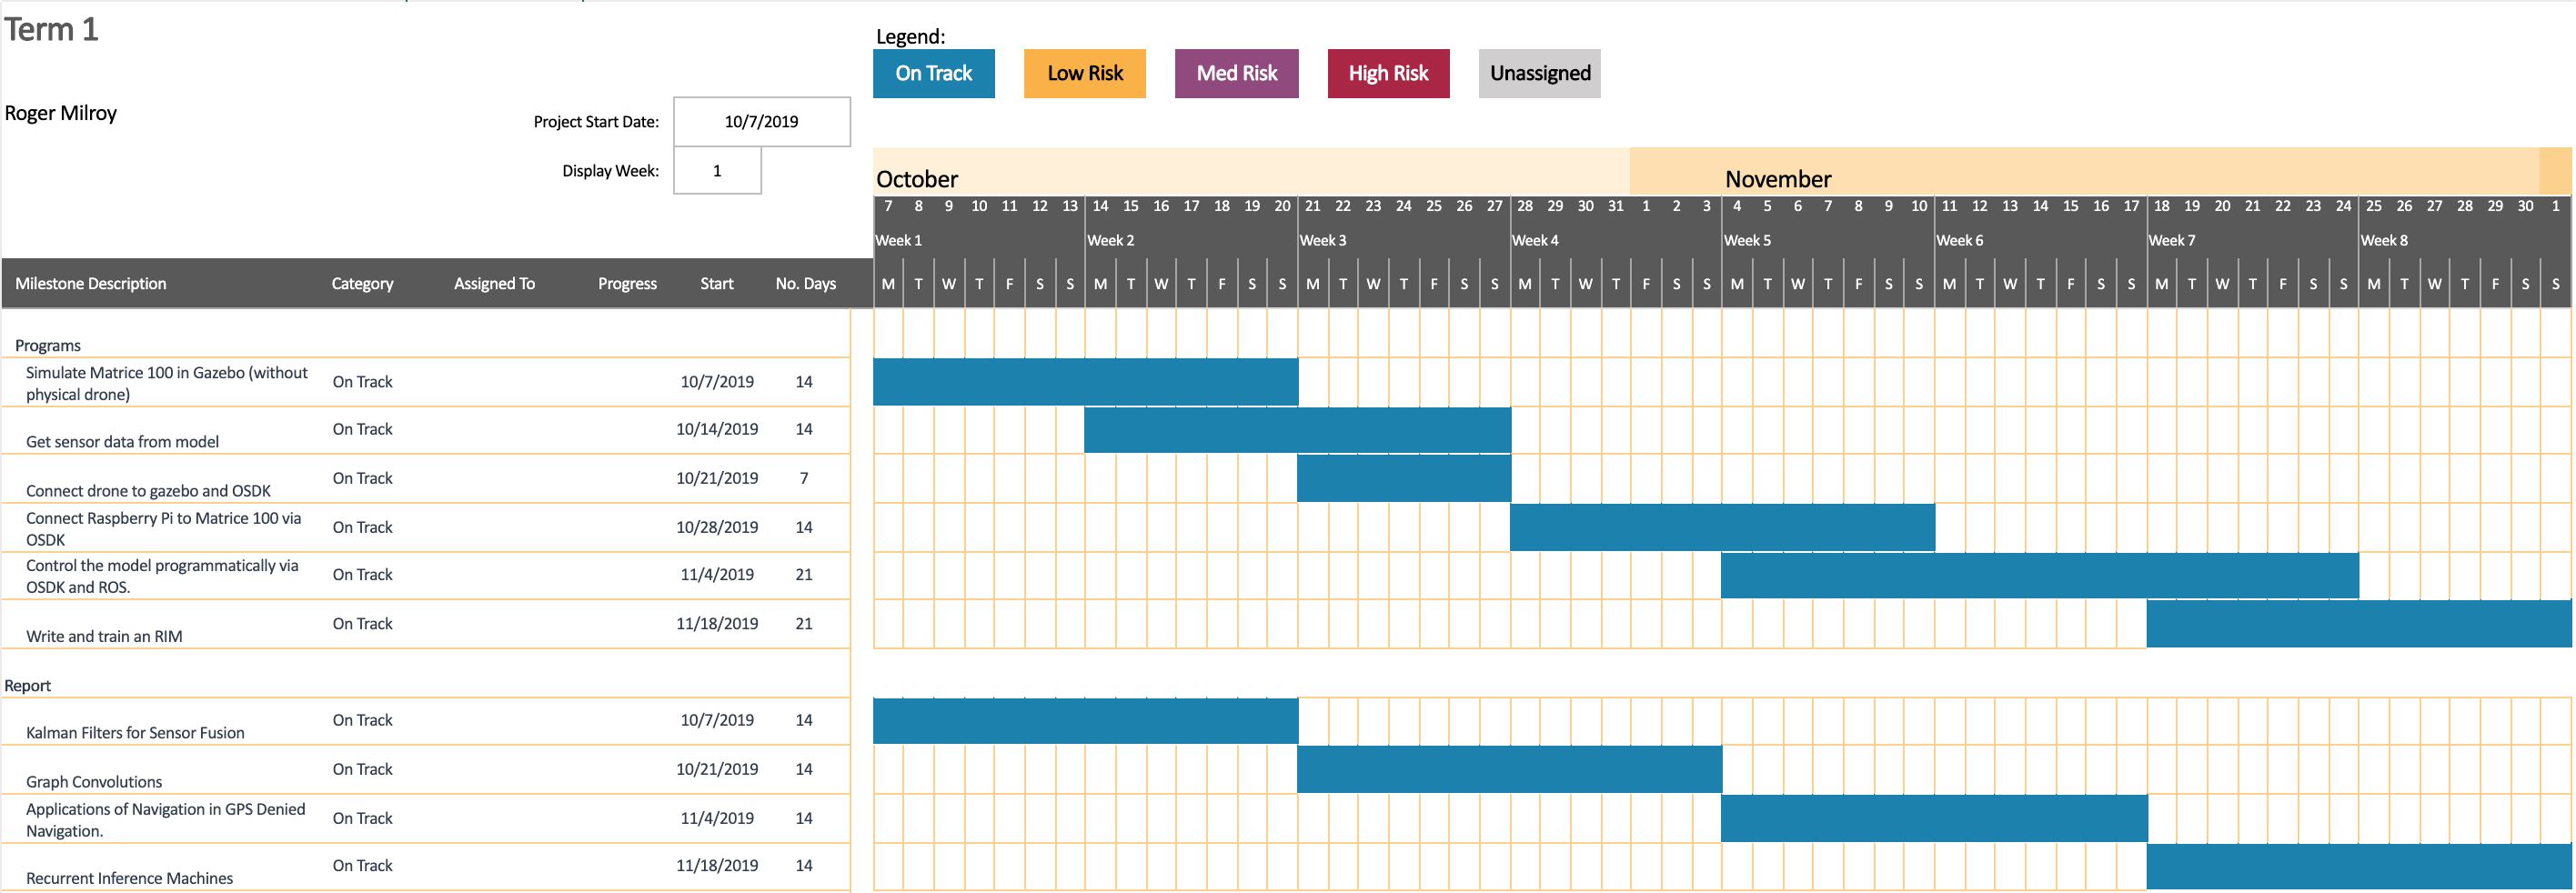
\includegraphics[width=\textwidth]{Term1Ganttv1.png}
  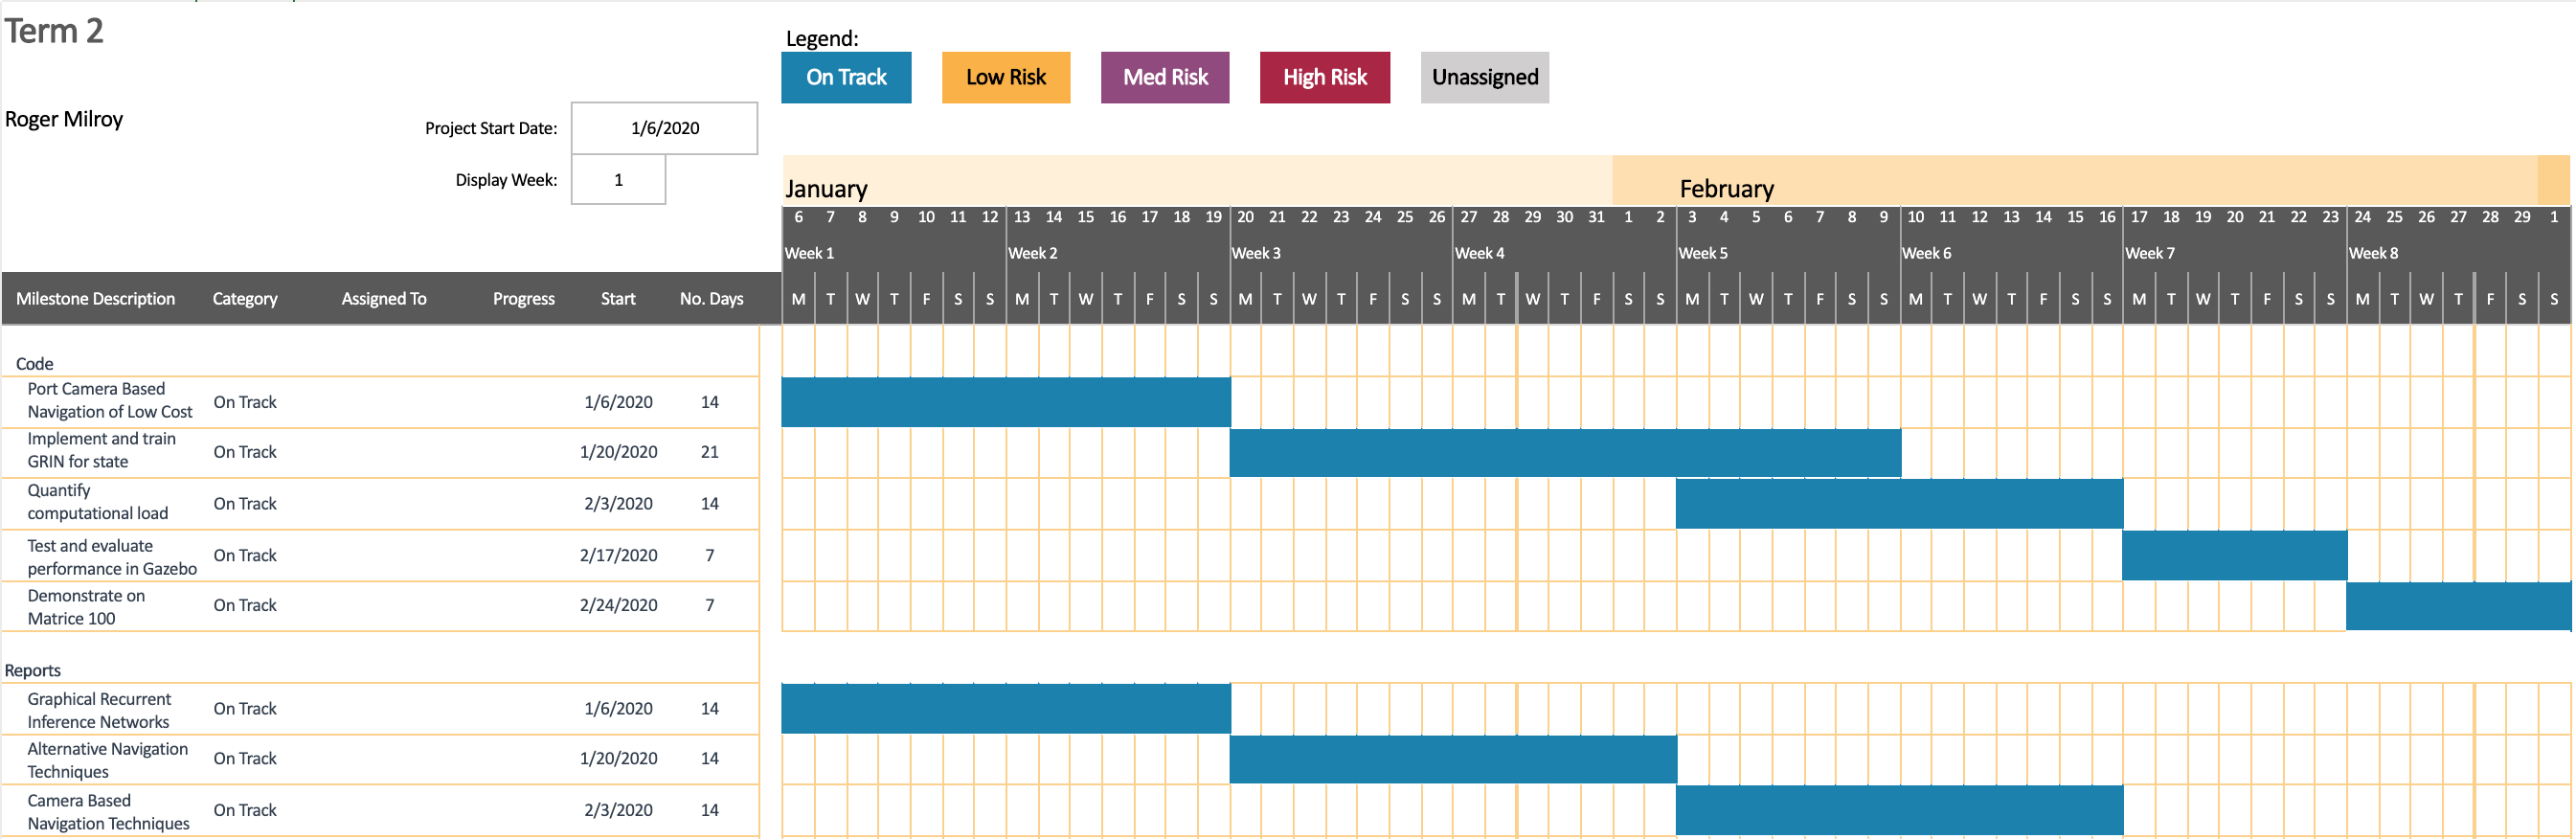
\includegraphics[width=\textwidth]{Term2Ganttv1.png}
  \caption{Original Plan Gantt Charts}
  \label{}
\end{figure}

\pagebreak

\section{Revised Plan}

While working on the project the outlook changed quite significantly when I found the code for the Monocular SLAM with scale recovery was open source and written with ROS. This meant that I could directly build upon their work and extend it instead of spending a large part of the project reimplementing their technique. This enabled me to pivot to focusing more on the implementation of HI as well as making the overall amount of work more reasonable. Under the new plan most of the first term was spent getting simulation working with the existing code base. I also implemented a simple version of the HI technique on synthetic position data.

The second term then focused on translating the proof of concept into a fully working system simulated in Gazebo. I also allocated time for working on enablers for the extension goal of deplying onto the DJI Matrice.


\begin{figure}[h]
  \centering
  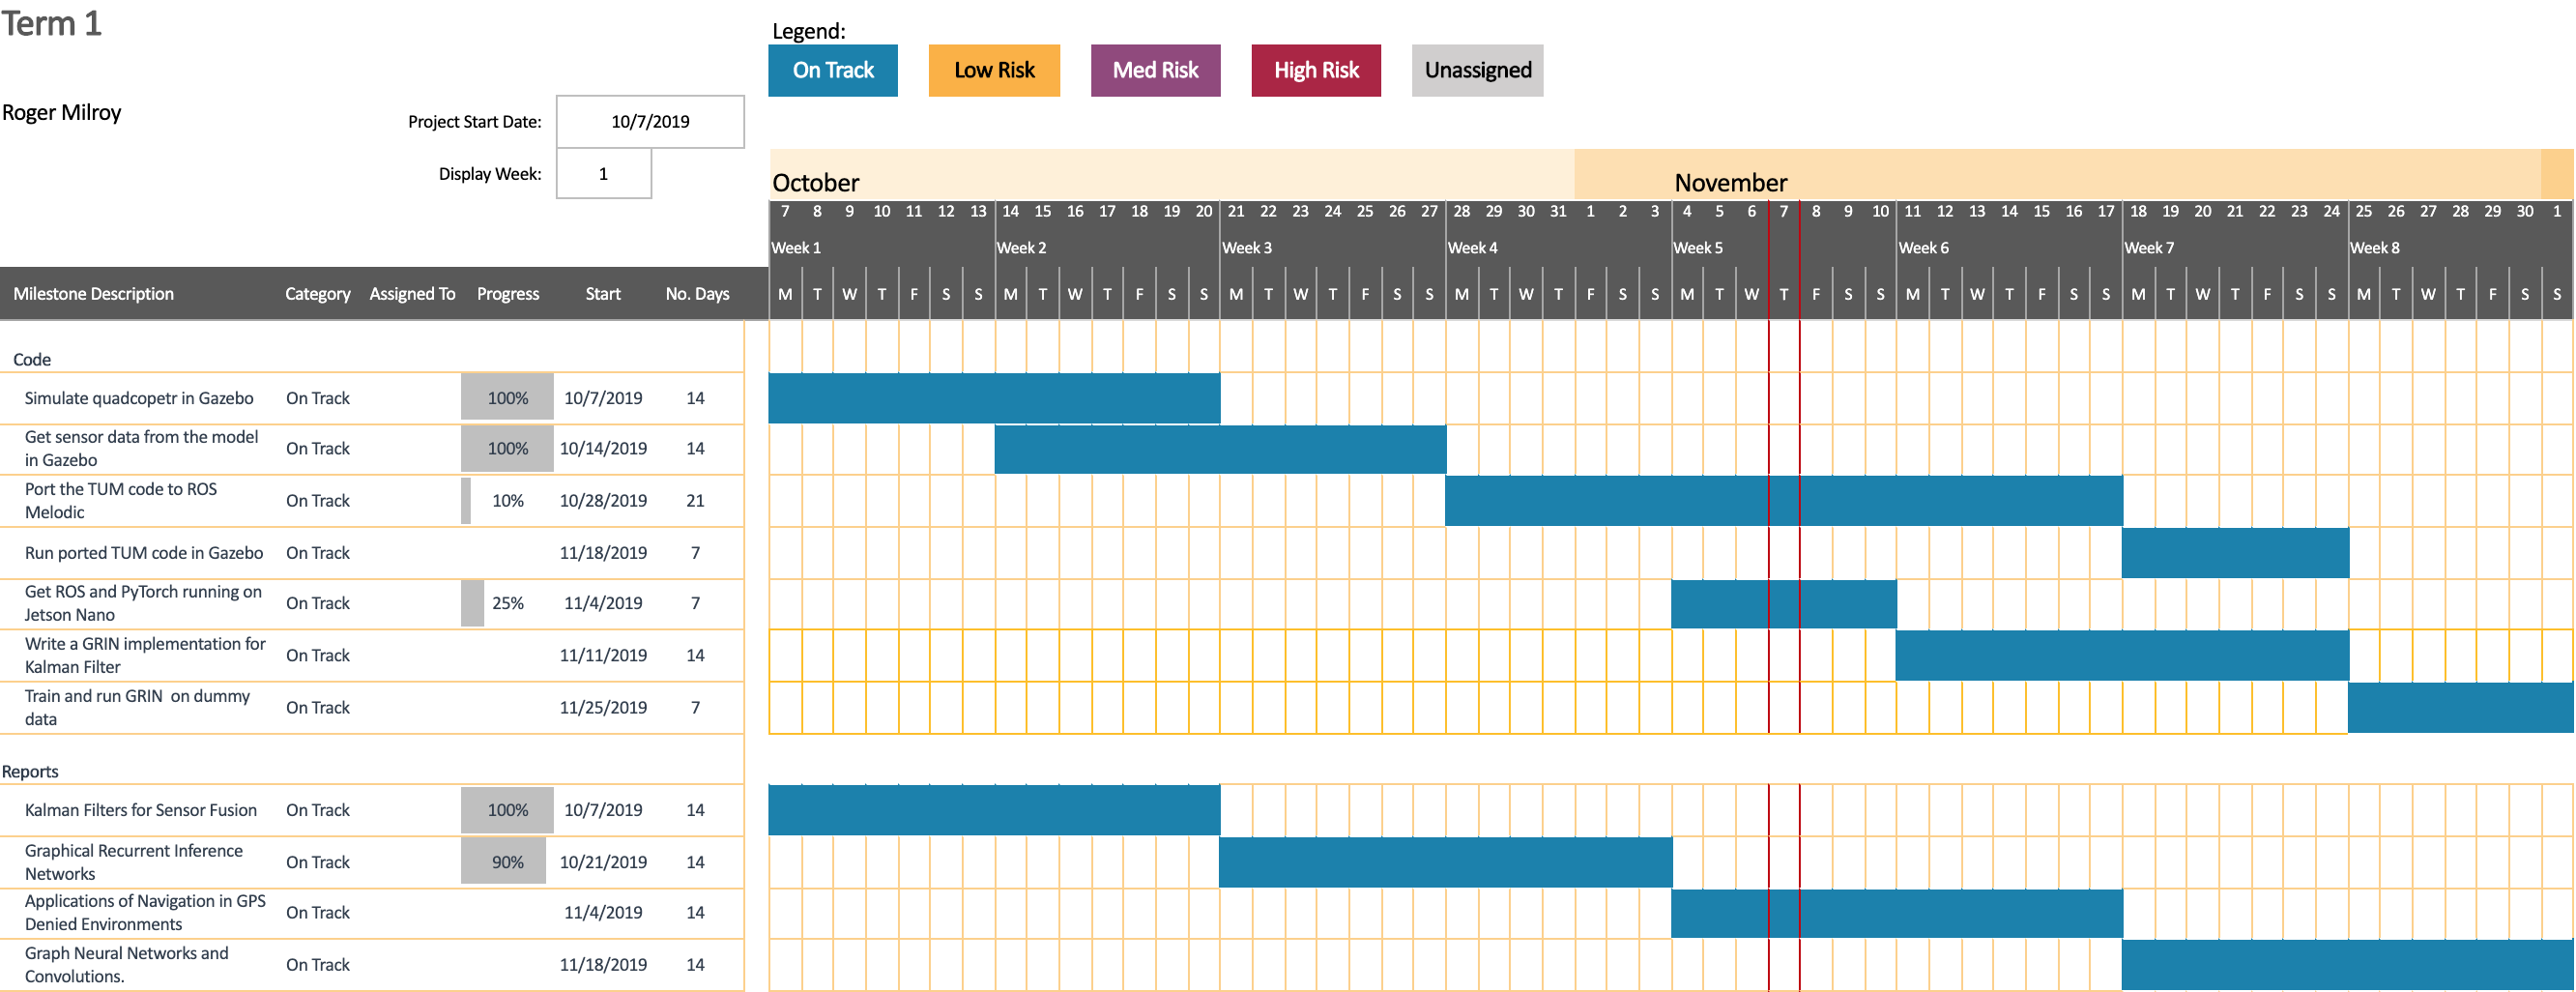
\includegraphics[width=\textwidth]{Term1GanttChart.png}
  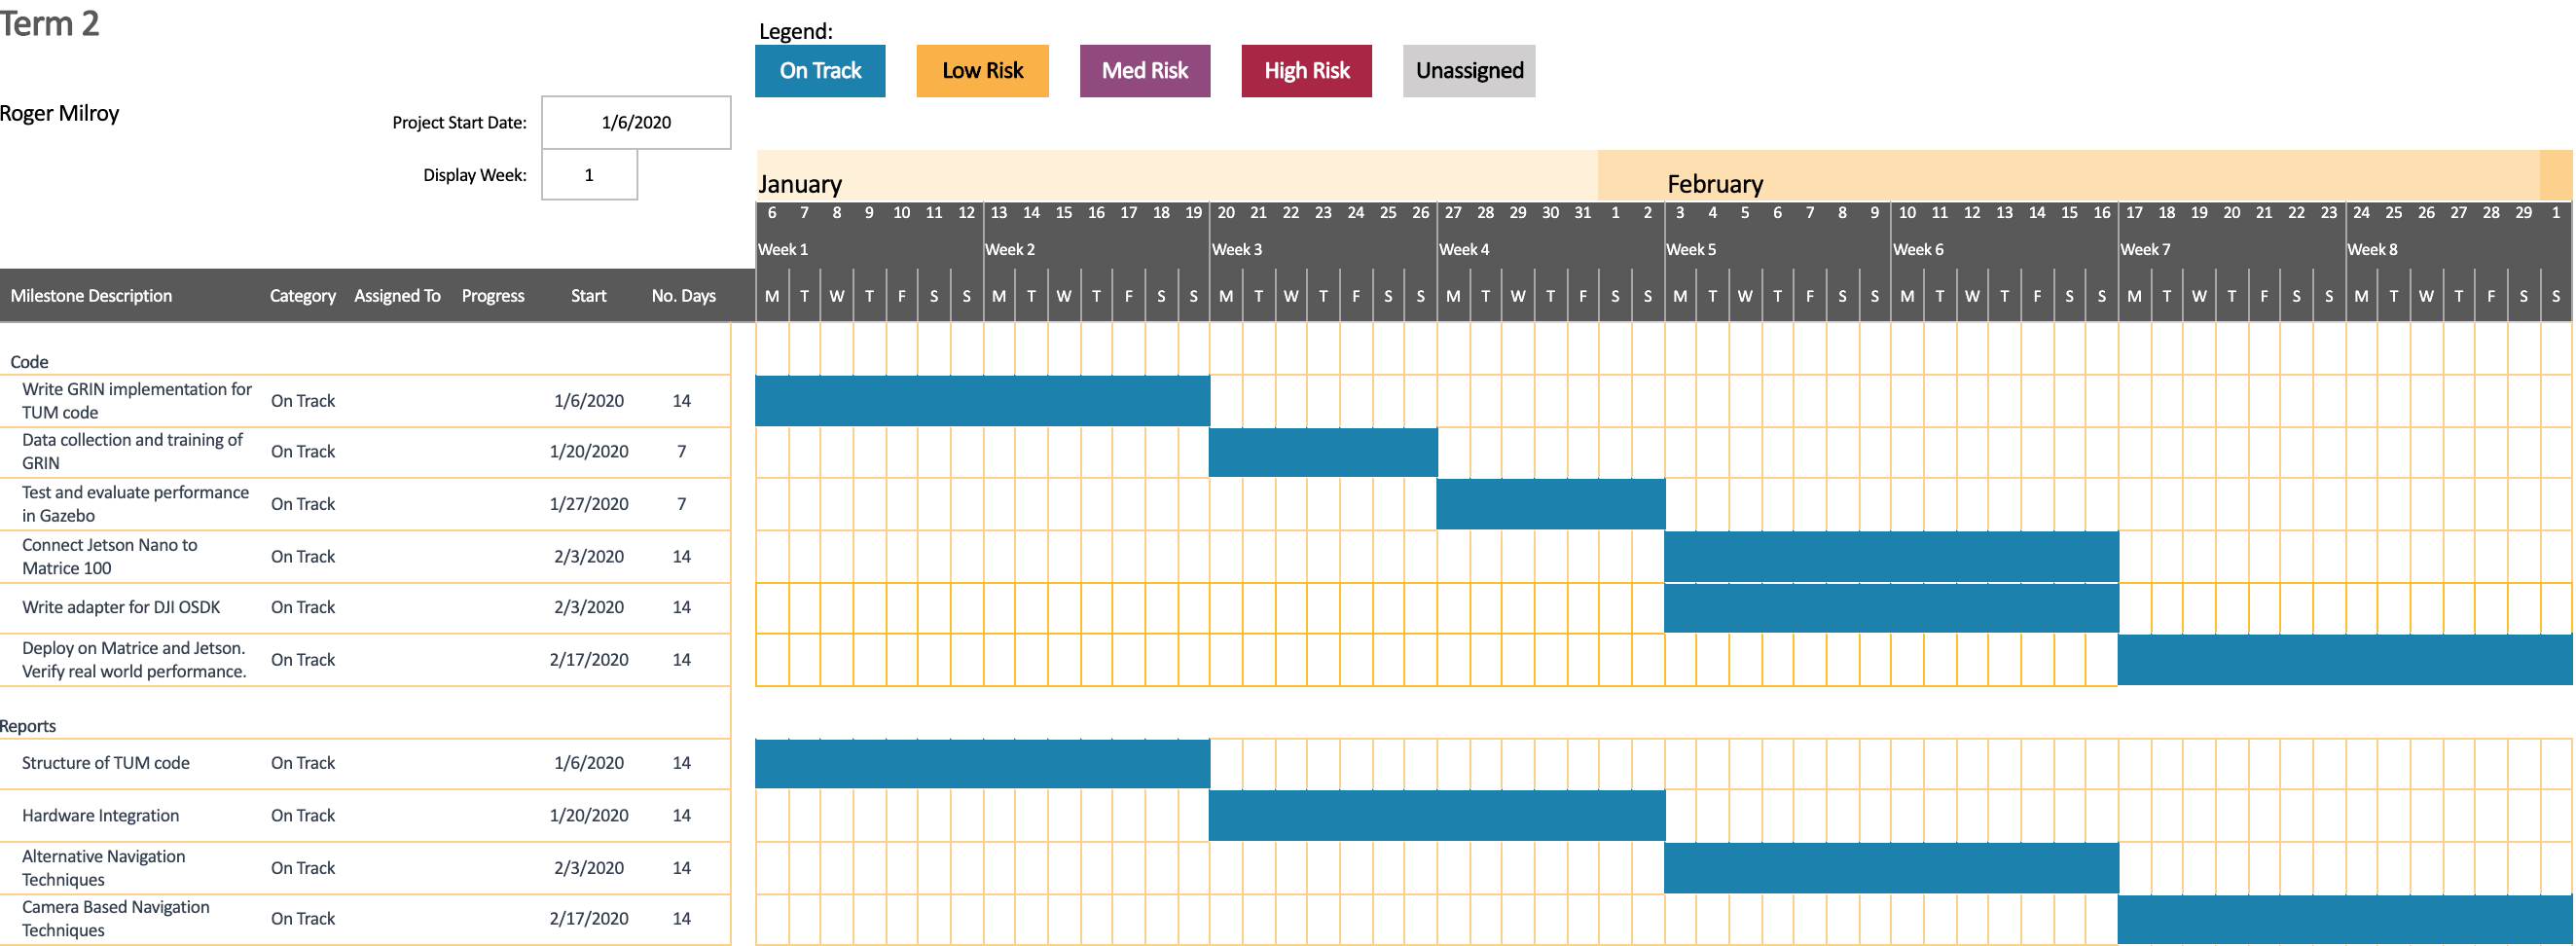
\includegraphics[width=\textwidth]{Term2GanttChart.png}
  \caption{Revised Plan Gantt Chart}
  \label{}
\end{figure}

%%%%%%%%%%%%%%%%%%%%%%
%%% Background Theory
\chapter{Background Theory}

\section{Gazebo and ROS}

%% Explainer on Gazebo and ROS and see if there are references for them.
In order to demostrate the effectiveness of the code that I have written it is essential that it is demonstrated first in a simulated environment. This neccesitates using Gazebo as it is the industry standard robot simulation software. In a similar token the industry standard robot development framework is ROS, which works with Gazebo and so this is the primary technology stack that I am using.

Both ROS and Gazebo are very powerful but they don't have a particularly easy onboarding process. For learning basic ROS concepts I used a service called Robot Ignite Academy that has some simple tutorials to make the process of learning the ROS way of doing things a bit quicker. One challenge I had at the very early stages was understanding what ROS actually was. There are very few high level descriptions of it, and they are certainly not the first topic on the ROS tutorials pages.

What I learned was that ROS is a paradigm of programming robots as well as an implementation of that paradigm. The paradigm is that of distributed programming where a system is composed of nodes that communicate to perform complex tasks. In this paradigm, Topics are communication channels that operate on the Publisher-Subscriber pattern, that are used by nodes to communicate between themselves \cite{ros_topics_2019}. Some nodes only read and some only publish. Nodes can also directly effect change in the robot, think of a node that controls a motor, it would read and change the voltage to the motor.

The other concepts that make up ROS are that of Services \cite{ros_servicess_2019} which are synchronous and Actions that are asynchronous, both operate on the Client - Server pattern.  And Messages \cite{ros_messages_2016} which actually have quite a bit of intricacy and can be quite confusing. There are 3 types of Message. Regular Messages that are published to Topics. Then Actions and Services also define their own formats of messages. They will often use standard messages defined for use in Topics but additional message formats will be generated for each Action or Service.

\section{Monocular SLAM with scale recovery.}

In two related papers \cite{Engel:FigureFlying}\cite{Engel:Camera-basedNav}, Engel et al. present a technique of Monocular SLAM that is able to recover absolute scale. In order to understand why this is significant and important some background is needed.

The primary problem of visual SLAM techniques is that of creating a high quality depth map of the surroundings. This can be accomplished by stereo vision, which is where two cameras are used and the distance and rotation between the two of them are known. Ideally the axes are aligned and there is no rotation between the cameras though this can vary depending on the specific requirements.This can be extended to use three or more cameras but in the more general case, known as structure from motion, it is possible to use a single camera. In that case we are trying to recover the transformation and rotation between frames. This is possible however it is not possible to recover absolute scale from this technique as we don't know the absolute distances between frames. In the stereo case the information about the position and orientation of the cameras relative to each other is known a priori and so we can recover absolute scale.

Engel et al. tackle the issue of scale recovery by using data from the IMU which usually consists of 3 accelerometers and 3 gyroscopes and often a magnetometer or other absolute scale sensors such as altimeter or barometer. This is standard equipment on quadcopters as it is needed to maintain stability. They use the information provided by this sensor in conjunction with the structure from motion equations in order to recover the absolute scale. In order to estimate the scale factor which is usually referred to as $\lambda$ they take a maximum likelihood approach, which in simple terms means they estimate the $\lambda$ that maximises the likelihood of the $x$ and $y$ positions measured by onboard sensors. In order to solve successfully they turn it into the negative log likelihood which you then minimize. This is a common trick and in this case it leads to a closed form solution for $\lambda$. This is important as it reduces the computational cost and makes it more feasible with onboard computation. In the paper they use a Parrot AR drone which has very constrained payload and computation capacity so they use offboard computation.

In the second paper \cite{Engel:FigureFlying} they present the full system including the scale estimation and demonstrate its effectiveness in position flying and holding.


\section{State Estimation}

%% Kalman Filters
The main method used for state estimation in the face of noisy sensors is the Kalman Filter. It is used in its non linear form, the Extended Kalman Filter (EKF), by Engel et al.\cite{Engel:Camera-basedNav} for state estimation and sensor fusion which are its most common uses in this field.

Let us formally define the problem. The system we are measuring is assumed to be characterised by a Hidden Markov Model, this is how Kalman characterised the dynamical system we are interested in \cite{Kalman1960ANA}. In this formulation there are hidden states $x$ and observations $y$. The system being a Hidden Markov Process means that it is characterised by the following equations:

\begin{align}
  x_t &= Ax_{t-1} + Q_t \\
  y_t &= Hx_t + R_t
\end{align}

Where $A$ is the transition matrix from time $t-1$ to $t$, and $\xi_t$ is the noise at time $t$. This represents that the model dynamics are stationary so $A$ is fixed but there is noise in transitions, that is transitioning between states is non-deterministic. $H$ is the measurement matrix and $R_t$ is the noise in the measurements. This models the reality of noisy measurements that may not be correct and in fact represents the true problem. We want to recover the true measurements despite being given noisy observations.
 
The Kalman Filter gives an optimum estimate of $x$ denoted as $x^*$ by deriving three matrices 
$\Phi^*$, $P^*$ and $\Delta^*$:

\begin{align}
  \Delta^*(t) &= A_{t+1;t}P^*_tH^T_t[H_tP^*_tH^T_t]^{-1} \\
  \Phi^*_{t+1;t} &= A_{t+1;t} - \Delta^*_{t+1;t}H{t} \\
  P^*_{t+1} &= \Phi^*_{t+1;t}P^*_tA^T_{t+1;t} + Q{t}
\end{align}

\pagebreak
Note that in the Kalman formulation he also considers non stationary dynamic systems. In our situation we assume stationarity which allows us to drop the time specification on the transition matrices $A$ and $H$.

With these matrices, the optimal estimate of state at time $t+1$, $\hat{x}_{t+1|t}$ is given by 

\begin{align}
  \hat{x}_{t+1|t} &= A^*\hat{x}_{t|t-1} + \Delta^*_ty_t
\end{align}

The estimation error $x'$ and covariance of the error, cov $x'$ are

\begin{align}
  x'_{t+1|t} &= A^*x'_{t|t-1} + Q_t \\
  \text{cov } x' &= P^*_t
\end{align}

From this we can see that the Kalman Filter is an iterative process where each iteration builds upon the previous best estimate of state. To recover the estimates of the true measurements we simply need to multiply the best estimates of the state by the measurement matris $H$.

Kalman and Bucy extended the Kalman filter that, in the form stated above works for discrete time, to the continuous case the year after the original paper \cite{Klmn1961NewRI}.

These equations only apply to linear dynamic models which is something of an issue given that most real life applications are of non linear dynamic systems. To solve this we use Taylor expansions to linearise our non-linear models around the current state \cite{ExtendedKalmanNasa}. This does unfortunately add a large overhead as we need to re linearise at each time step to avoid accumulating linearisation errors.

%% Graph Neural Networks
\section{Graph Neural Networks}

% Explain the premise behing GNNs
As the technique I am implementing makes use of Graph Neural Networks (GNNs) I will first explore what GNNs in relation to regular neural networks (NNs). If you are already very familiar with NNs feel free to move on to the next section.

\subsection{Neural Networks}
To understand GNNs it is first necessary to understand some basic things about NNs and some of their properties. Firstly the paradigm of learning that NNs fall under to is called representation learning. That is learning meaningful representations of data in service of a task.

Secondly is that NNs are Universal Function Approximators \cite{Hornik}. That is given sufficient hidden layer neurons a neural network can approximate any real valued function no matter how complex. This is the basis for their power and flexibility.

This doesn't come without drawbacks however. The cost of this flexibility is that training a universal function approximator (or a feed forward network with an arbitrarily large hidden layer) is not necessarily feasible in computational terms or in terms of the amount of data required. 

In order to overcome this limitation there has been great progress in formulating specific architectures of neural networks. Some good examples of these are Convolutional Neural Networks (CNNs) and Residual Networks (ResNets). One of the keys to these models successes is that they constrain the neural architecture. For these two in particular they constrain the model to Euclidean space and particular dimensions within this space. This restriction means that the resulting network is no longer a universal function approximator but that also reduces the amount that the network has to learn for example the rules of Euclidean space and what a dimension within the data is. It is precisely these restrictions that enable such networks to learn with fewer data samples and to a greater accuracy than would be possible otherwise.

This can be rephrased with a slightly different interpretation by seeing the constraints on the network as introducing inductive biases into the model. This biases the network to learn certain features of the dataset and not others. 

\subsection{Graphs}

In order to motivate GNNs a little more fully I briefly outline some basics of Graphs and Graph Theory. If you are familiar with Graphs then feel free to proceed directly to the GNN section.

% Define Graphs?
We define graphs as a collection of nodes (also known as vertices though I will use the word node from now on) and a collection of edges over those nodes. Graphs are prevalent across many different areas of science and are a particular focus of many Computer Scientists. Famous examples of graph algorithms include Djistra's Algorithm, Depth First Search and A star. Why are graphs so prevalent? Well the answer is that they have great expressive power to represent objects or concepts and their relations.

The flexibility of graphs is mirrored in the great variety of operations that we might want to carry out over them. At the same time there is a huge number of different configurations of graphs varying over degree of connectivity of each node, whether edges are weighted or directed, containing cycles or not and whether the graph changes at all. Whether the edges represent different kinds of relation and what information each node contains.

\subsection{Graph Neural Networks}

A quick note on representation.

We consider each node to have a vector label or feature. This may contain information about edges or not. If we were to try and apply CNNs or RNNs to graphs in this form, we could do so by stacking the node features and operating over that. In this case the node features would contain the information about edges.

This is not ideal because it enforces or biases the model to a particular ordering of nodes where there might not be one. We could overcome this by computing over all possible orderings of nodes. This would however add significant computation. \cite{graphoverview}It also prevents the model from exploiting the graphs inherent structure, as it had been folded into the nodes themselves. It is clear then that this is not the best approach.

\pagebreak
% GNN
\subsubsection{Original GNN}

Now I will explain the original GNN proposed in \cite{GNN}. The following explanation is drawn from \cite{graphoverview} with some rewording. The goal of the GNN is to learn an embedding $ \emph{h}_x \in \Reals_s $ of each node $x$ which contains the information from the node and its locality. This embedding is then used to generate an output $\emph{o}_x$ of each node, often called the decoding step,where the embedding of each node generates a prediction of some kind for example the node labels.

In order to compute these embeddings and outputs we define two parametric functions, the first is $f$ a local transition function which is shared by all nodes, and $g$ the local output function. These are defined as:

\begin{align}
  \textbf{h}_v &= \emph{f }(\textbf{x}_v, \textbf{x}_{co[v]}, \textbf{h}_{ne[v]}, \textbf{x}_{ne[v]})\\
  \textbf{o}_v &= \emph{g }(\textbf{h}_v, \textbf{x}_v)
\end{align}

where $\textbf{x}_v$, $\textbf{x}_{co[v]}$, $\textbf{h}_{ne[v]}$, $\textbf{x}_{ne[v]}$ are the features of v, the features of its edges, the states, and the features of the nodes in the neighborhood of $v$, respectively.

This can be condensed by stacking vectors to form matrices. Then we have $\textbf{X}$, $\textbf{X}_N$, $\textbf{O}$ and $\textbf{H}$ consisting of all features, the features of the nodes, the outputs and the states respectively. In this form we then have global transition function $F$ and global output function $G$.

\begin{align}
  \textbf{H} &= F(\textbf{H}, \textbf{X})\\
  \textbf{O} &= G(\textbf{H}, \textbf{X}_N)\\
\end{align}

The GNN takes inspiration from Banach's fixed point theorem \cite{khamsi_kirk_2011} and uses the following iterative scheme to compute the states:

\begin{align}
  \textbf{H}^{t+1} = F(\textbf{H}^t, \textbf{X})
\end{align}

This converges to a stable $H$ exponentially fast for any start point of $\textbf{H}_0$

We use NNs for the parameterised functions $\emph{f}$ and $\emph{g}$.

As stated in \cite{GGNN} the model is trained using the Almeida-Pineda algorithm \cite{Almeida}\cite{Pineda} where the states are computed to convergence at which point the output and losses are computed. The gradients of the weights in the transition function and output fuction networks are computed from this final state and the weights updated according to the optimisation algorithm selected.


% Adding Recurrence.
\subsubsection{Recurrence}

An extension or variation of the GNN is the Gated Graph Neural Network (GGNN). The key reason for the introductionof the GGNN is to reduce the restrictions on the transition function. Rewording what was stated in \cite{GGNN} the paper that proposes the GGNN they outline the challenge of the original GNNs learning scheme. As I just described, in the regular GNN the loss and gradients are computed relative to the final converged state. This requires that the parameters of the NNs be constrained so that it is a contraction map, otherwise convergence cannot be guaranteed. In order to remove this restriction, as there is evidence that long range dependencies ar lost in the contraction map scheme, they add a Gated Recurrent Unit (GRU) \cite{GRU}. In this situation information is conserved at each time step and while gradients are still computed from the final state and output, the GRU is unrolled backpropagated through time (BPTT) \cite{Pineda} is used to propagate these gradients across all time steps of the iterative procedure. This removes the constraint on the parameters of the component NNs.


% MPNN
\subsubsection{MPNN}

After the introduction of the GNN there have been many additional variants have been proposed such as Spectral Networks and Graph Convolutional Networks (GCN) and Graph Attention Networks.

There have been proposed some frameworks that generalise these various variants of GNNs. The framework relevant to this application is called the Message Passing Neural Network (MPNN) which was proposed by \cite{mpnn}.

Again I am using the explanation of \cite{graphoverview} with some rewording as it is an excellent high level explanation.

The MPNN has two phases, the message passing phase and the readout phase. The message passing phase runs for $T$ steps and there are two parts the message function $M_t$ and the update function $U_t$, $\textbf{e}_{vw}$ is the edge feature on the edge from $v$ to $w$.

\begin{align}
  \textbf{m}^{t+1}_v &= \sum_{w \in N_v} \emph{M}_t(\textbf{h}^t_v, \textbf{h}^t_e, \textbf{e}^t_{vw})\\
  \textbf{h}^{t+1}_v &= U_t(\textbf{h}^t_v, \textbf{m}^t_v)
\end{align}

The readout phase computes a vector for the whole graph using the readout function $R$ and $T$ denotes the total number of time steps or iterations.

\begin{align}
  \hat{\textbf{y}} &= R({\textbf{h}^T_v | v \in G})
\end{align}

This is modifiable of course to allow a per node output. In this case the readout function would be similar to the output function of the original GNN. In fact there are many parallels between the original GNN and the MPNN but the MPNN has more flexibility which allows it to capture the majority if not all of the supervised variants of the GNN.

We can also implement the GGNN using this framework.

\pagebreak
%% Hybrid Inference
\section{Hybrid Inference}

Now I introduce the technique that form the core objective of this project, Hybrid Inference. First introduced in \cite{Satorras2019CombiningGA} which also gave examples on Lorenz attractors and Kalman filters. While Kalman Filters give optimal estimates in the face of noise, it is almost impossible for them to be completely precise due to that noise. This we can see by observing the error in the estimates at each time step.

Absent an accurate fix of state, ie. a noiseless measurement, the error grows continuously to the point where estimates may no longer be meaningful.

At the same time it is now possible to train a neural network to directly estimate position given noisy inputs \cite{NNStateEstimation}. The concept of Hybrid Inference is to leverage the relative strengths of pre-existing knowledge, in this case the Kalman Filter that accurately describes the behaviour of linear or linearised dynamic models up to a degree of error, and Deep Learning techniques that are able to model highly non linear systems but require large amounts of data to train. In the Hybrid Inference model, expert knowledge is incorporated by integrating the model of the system with a Graphical Neural Network (GNN) modelling the residual error to improve accuracy above what is possible with a Kalman filter alone.


Reexamining the problem solved by the Kalman filter, Satorras, Akata and Welling reformulate the problem to be a maximum likelihood problem \cite{Satorras2019CombiningGA}. Where the states are $\mathbf{x} = \{x_0, x_1 ... x_k\}$ and the observations are $\mathbf{y} = \{y_0, y_1 ... y_k\}$ In this context, the task is to predict the optimal estimate of $\mathbf{x}$, $\mathbf{\hat{x}}$ which is defined as

\begin{align}
  \mathbf{\hat{x}} = \underset{x}{\text{argmax}}\ p(\mathbf{x}|\mathbf{y})
\end{align}

Again as we assume a Markov process and that the transition is stationary this can be expressed as 

\begin{align}
  p(\mathbf{x},\mathbf{y}) = p(x_0)\prod_{t=1}^T p(x_t|x_t-1) p(y_t|x_t)
\end{align}

They model this as an iterative optimization process to arrive at $\mathbf{\hat{x}}$ Specifically they define a recursive update operation for the general case and then formulate it 
for the Hidden Markov case

\begin{align}
  x_t^{(i+1)} = x_t^{(i)} + \gamma M_t
\end{align}

Where $M_t$ represents the sum of matrix products, which they call messages, from $x_t-1$ to $x_t$ from $x_t+1$ to $x_t$ and from $y_t$ to $x_t$.

In our case these messages turn out to be

\begin{align}
  x_{t-1} \rightarrow x_{t} &= -Q^{-1}(x_t - Fx_{t-1}) \\
  x_{t+1} \rightarrow x_{t} &= F^TQ^{-1}(x_{t+1} - Fx_t) \\
  y_t \rightarrow x_t &= H^TR^{-1}(y_t - Hx_t) 
\end{align}

The graphical interpretation is of the $x$s and $y$s at each time step forming nodes in a graph. The edges are the same as the direction of the messages, that is from $x_{t-1} \rightarrow x_t$, $x_{t+1} \rightarrow x_t$ and $y_t \rightarrow x_t$. The messages passed over these edges iteratively update the $x$s and after some iterations they converge to a best estimate.

%% Insert a graph here.

\begin{figure}[h]
  \centering
  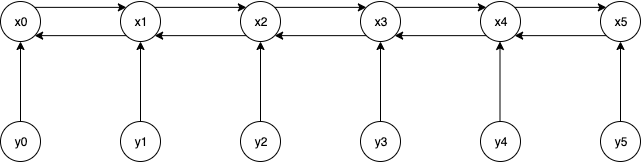
\includegraphics[width=0.8\textwidth]{GraphicalKalmanModel.png}  
  \caption{Graphical Representation of the Kalman Filter}
  \label{}
\end{figure}

This graphical interpretation allows us to define an equivalent graph with different dimension nodes but the same edges. These are known as $h_x$ and $h_y$ which stands for hidden nodes relating to $x$ and $y$ respectively. 

%% Insert another graph here.

The key part of the paper is to define an MPNN that operates over this graph with a message passing routine over the nodes that connect edges and the messages passed in the original graph. More specifically for each type of edge, for example $y_t \rightarrow x_t$, we define a feedforward neural network that takes the source node, the target node and the message and outputs an encoding of the edge, I will refer to these as edge models. This corresponds to the Message function of the MPNN. These encodings are summed according to their source node and then passed through a separate feedforward network which I will call the node model. This corresponds to the Update function.

The output of this is passed through a GRU along with the previous $h_x$ in order to produce a new estimate of $h_x$. The interpretation of this is that edge feedforward networks compute the residual error over the edges, the node model computes the residual error left in the $h_x$ and the GRU allows some of the past residual error to propagate into the current estimate. The final step passes the new $h_x$ through a decoding step to produce an additional corrective factor in addition to $M_t$ called $\epsilon$.

This gives us the final general recursive update rule

\begin{align}
  x_t^{(i+1)} = x_t^{(i)} + \gamma (M_t + \epsilon_t)
\end{align}


\section{My Contributions}

% Some discussion of what I have accomplished. 
% from the booklet "an interesting discussion on what you have achieved in a more global context"

In the HI paper they implement a Kalman Smoother over linear and non linear systems however in both of these cases they didn't cover the case of having inputs to the system,  using the technique for prediction or a true Extended Kalman Filter implementation.

Inputs are often used as they allow the algorithm to make the most accurate estimates due to having more information. This should be fairly self evident.

In order to use HI on MAVs in reality it is also necessary to be able to predict a short way into the future, that is to implement a true Kalman Filter rather than just a Smoother, the distinction is quite important, a Smoother operates only on timesteps prior to the current measurement and a Filter operates on the current measurement as well as future time steps without measurements (by omitting the update step). In order to control a drone effectively you need to account for the fact that there will be time lags in some parts of the system. For this reason you need to be able to predict a short way into the future for the most effective control.


% Change to the probability function
\subsubsection{Inputs}

To add inputs I needed to change the probability distribution we are modelling.

\begin{align}
  \hat{\textbf{x}} = \underset{\textbf{x}}{\text{arg max }} p(\textbf{x} | \textbf{y}, \textbf{u}) 
\end{align}
where $\textbf{u}$ are the inputs.

This changes the recursive update function (Eq. 5 in \cite{Satorras2019CombiningGA}) to be 

\begin{align}
  \textbf{x}^{(i+1)} = \textbf{x}^{(i)} + \gamma \nabla_{\textbf{x}^{(i)}}log(p(\textbf{x}^{(i)} | \textbf{y}, \textbf{u}))
\end{align}

% Change to the messages

Which in turn changes the derived input messages to be 

\begin{align}
  \mu_{x_{k-1} \rightarrow x_k}^{(i)} &= \frac{\partial}{\partial x_k^{(i)}} log(p(x_k^{(i)}|x_{k-1}^{(i)}, u_{k})\\
  \mu_{x_{k+1} \rightarrow x_k}^{(i)} &= \frac{\partial}{\partial x_k^{(i)}} log(p(x_{k+1}^{(i)}|x_{k}^{(i)}, u_{k})\\
  \mu_{x_{y_k} \rightarrow x_k}^{(i)} &= \frac{\partial}{\partial x_k^{(i)}} log(p(y_{k}|x_{k}^{(i)})
\end{align}

% Change to the derived matrix operations.

Formulated for the Kalman filter model this gives us

\begin{align}
  \mu_{x_{k-1} \rightarrow x_k}^{(i)} &= -\textbf{Q}^{-1}(x_k - (\textbf{F}x_{k-1} +\textbf{G}u_k))\\
  \mu_{x_{k+1} \rightarrow x_k}^{(i)} &= \textbf{F}^T\textbf{Q}^{-1}(x_{k+1} - (\textbf{x}_k + \textbf{G}u_{k+1}))\\
  \mu_{x_{y_k} \rightarrow x_k}^{(i)} &= \textbf{H}^T\textbf{R}^{-1}(y_k - \textbf{H}x_k)
\end{align}

Where $\textbf{G}$ is the gain matrix over the inputs $u$.

In a wider context this is a small but significant extension that shows that this technique could be used in the full spectrum of applications of the Kalman Smoother. 

I detail the implementation in Work Completed and share the results which are comparable with the original HI implementation.

\pagebreak
% Extension to prediction.
\subsubsection{Prediction}

Extending to prediction is a different challenge. I elected to take the simplest approach which coincidentally is analagous to the approach that the KF takes for prediction.

I augment the sequence over which the technique operates for smoothing with $0$ values in place of measurements or $y$s. This ensures that the messages from $y_k$ for these values are also $0$ and ensures that all the information for estimating the $x$s at that point are from previous $x$s in the sequence.

This is best understood graphically. Figure 3.2 shows the graphical model when predicting one step ahead. As can be seen the final $y$ is replaced with a $0$ vector and so all the messages from that throughout the iterative procedure are also $0$ vectors.

\begin{figure}[h]
  \centering
  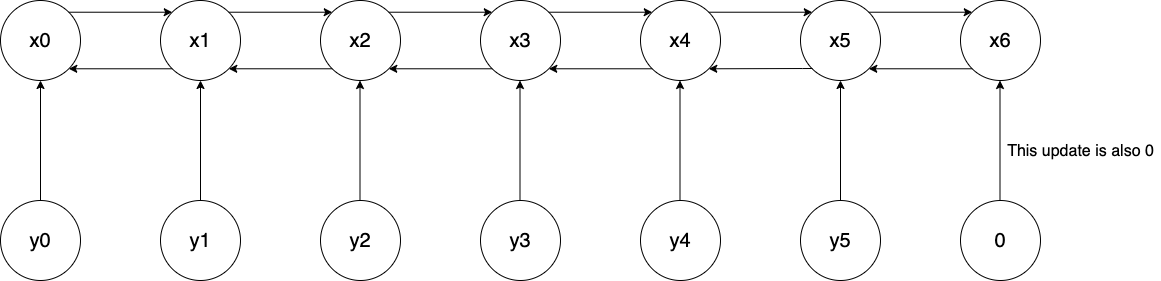
\includegraphics[width=\textwidth]{PredictionKalman.png}
  \caption{Graphical view of predicting one step ahead.}
  \label{}
\end{figure}

This is analagous to running the predict steps of the KF with no update step. The sequence is again iteratively optimized to arrive at the estimates of the future states.

%%% Software Engineering
\chapter{Software Engineering}

\section{Tools}

\subsubsection{Version Control System}

I used git as my version control system, and GitHub as my remote. I actually have a number of repositories because for the ROS section of the project it was necessary to modify existing projects code. I created a private fork of the relevant projects and then modified them as necessary.

I have separate branches for development, reports and for each feature that I am working on. These last ones are only temporary and are closed as soon as the feature is tested and integrated back into development. The workflow that I have decided upon is to use development for completed features once they have been tested. This does not imply that development is stable however so I only release code considered stable to master. The idea is that master should only contain stable code and be safe to use at any point.

\subsubsection{Project Task Tracking}

I used Trello in order to organise and keep track of tasks while completing them. I used a single board with To Do, Doing and Done lists. Each task is a card and has an associated due date. This is really useful to stay on track and quickly assess the state of the project at a glance. I also used this while replanning as I could evaluate each task and see whether it was still relevant in the new context. One additional advantage of using Trello is that it keeps track of history and has space for lists within tasks allowing them to be broken up into sub tasks.

\begin{figure}[h!]
  \centering
  
\includegraphics[width=\textwidth]{TrelloScreenshot.png}
  \caption{Trello}
  \label{}
\end{figure}


\subsubsection{Development Support Tools}

IDEs support efficient coding with a number of useful tools and features. The primary advantage is the code completion support. This greatly speeds development, especially in more verbose languages. One of the most valuable features in the context of this project is the debugger. This allows the developer to step through the program where necessary and inspect each variable as it changes. This was particularly useful in the implementation of HI as the dimensions of the tensors at each step is extremely important and often hard to keep track of. Interestingly this particular issue has caused PyTorch to add support for named tensors. This allows each dimension to be named, which mostly solves the problem. And is an interesting example of how the language or frameworks we use support or hinder development depending on the features they allow.

I used VSCode, CLion and PyCharm as Development Environments. They each have different advantages and disadvantages and I used VSCode and CLion for the C++ work and PyCharm for the Python work. The main advantage to VSCode is its flexibility and support for almost all languages given extensions. It's drawbacks stem from its flexibility however with slightly reduced abilities in all languages, at least in my experience. This led me to use CLion for the more serious C++ programming as it is more tailored to supporting C++ work. For the Python work I used PyCharm exclusively and it functioned excellently.

For ROS development I have an Ubuntu VM with the relevant dependencies installed as well as the IDEs I just mentioned. I used AWS instances where I needed more power than I had available locally. I generally used GPU accelerated instances running Ubuntu 18.04 for consistency with my local VM. ROS uses catkin for building projects which in turn builds upon CMake and I used UMLet for drawing up the UML diagrams 

For testing I used the built in testing framework for Python, 'unittest'. This provides a very similar framework to JUnit and allows for clear easy test setup and management.


\section{Design and Testing}

\subsection{Design}
% ROS

This project has been different to most projects that I have worked on to date in terms of software design. Most of these projects have been implemented from scratch using some different technologies but either very little or nothing in terms of pre existing code base. This gives a lot of freedom and control to the design.

In this project it has been quite different. I have been working with pre-existing code bases from TU Munich and TU Darmstadt. This has constrained the design and implementation of these parts of the project. Outside of these sections the goal of all the design decisions has been modularity and reusability. In some cases this has not been possible due to constraints of the technologies that I have been working with.

It is widely accepted that good code should be modular and reusable where possible. There are aspects where this is obviously not possible, such as configurations and any implementation specific work, but this should where possible be isolated and offer abstract interfaces.

With respect to the packages I have chosen, the hector stack and the TUM work, they have to some extent taken this approach but only really within the project. This complicated my work somewhat but at the same time using these as the base allowed me to explore more advanced concepts rather than reimplementing the functionality of these modules. It has forced me to adapt my natural coding style to fit in with the pre existing code and conventions established within them. 

For the HI implementation section of the project, I separated the Graphical and GNN parts of the implementation. They became separate classes that had defined interfaces for the forward methods that were as stable as possible. They are composed into the final HI implementation, this has risks of high coupling which I mitigated as far as possible by keeping the interfaces (primarily the forward method) as stable as possible in terms of inputs and return values. This allows the internal structure to change without the HI implementation being modified at all.

\begin{figure}[h!]
  \centering
  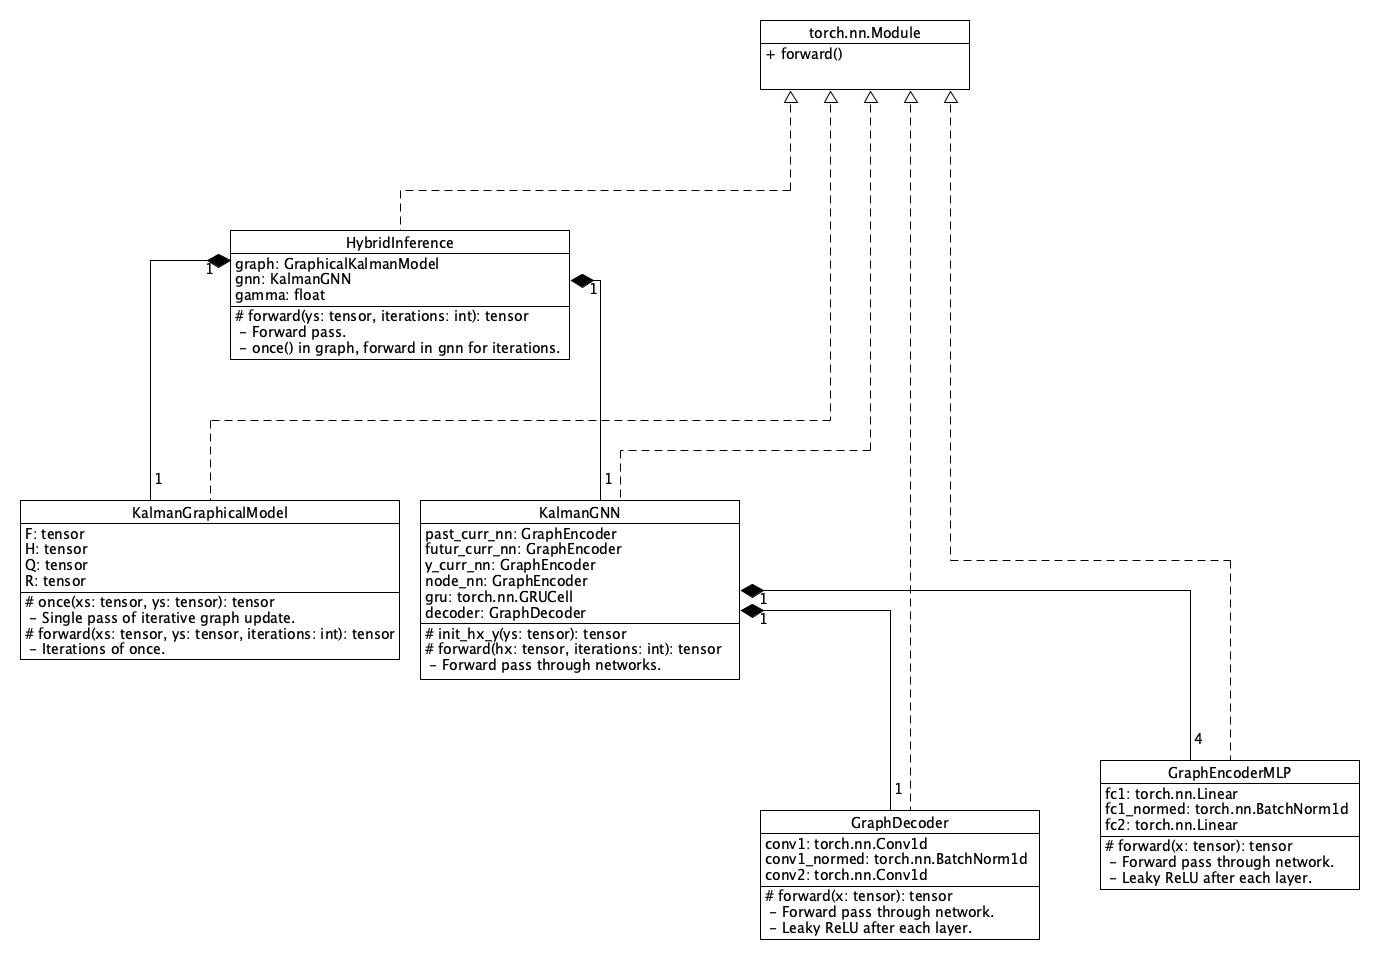
\includegraphics[height=0.36\textheight]{hybrid-inference-uml.png}
  \caption{Class diagram for Hybrid Inference}
  \label{}
\end{figure}

I added Predictor and Smoother interfaces in order to further enforce this principle. There are some limitations to this due to the fact that HI works with multidimensional tensors and dimensionality makes a large difference. I would ideally be able to prescribe the dimensionality of the inputs and return values from each function. Unfortunately there is no mechanism for that in any language or framework at this time.

When it came time to integrate HI into the hector stack I needed to port the PyTorch implementation of HI to run in C++. This required various changes to make the implementation serialisable with the TorchScript compiler module. Some of these overrode design decisions I had made earlier.

While integrating HI into the hector stack, I was much more restricted in the design choices I could make as I had to work inside the structure that was already established. Specifically I had originally planned to implement the HI as a ROS node to minimise coupling. The hector stack decided not to take that approach for pose estimation, I believe due to latency concerns. So I directly subclassed their Filter base class modelled on their EKF implementation.

\begin{figure}[h!]
  \centering
  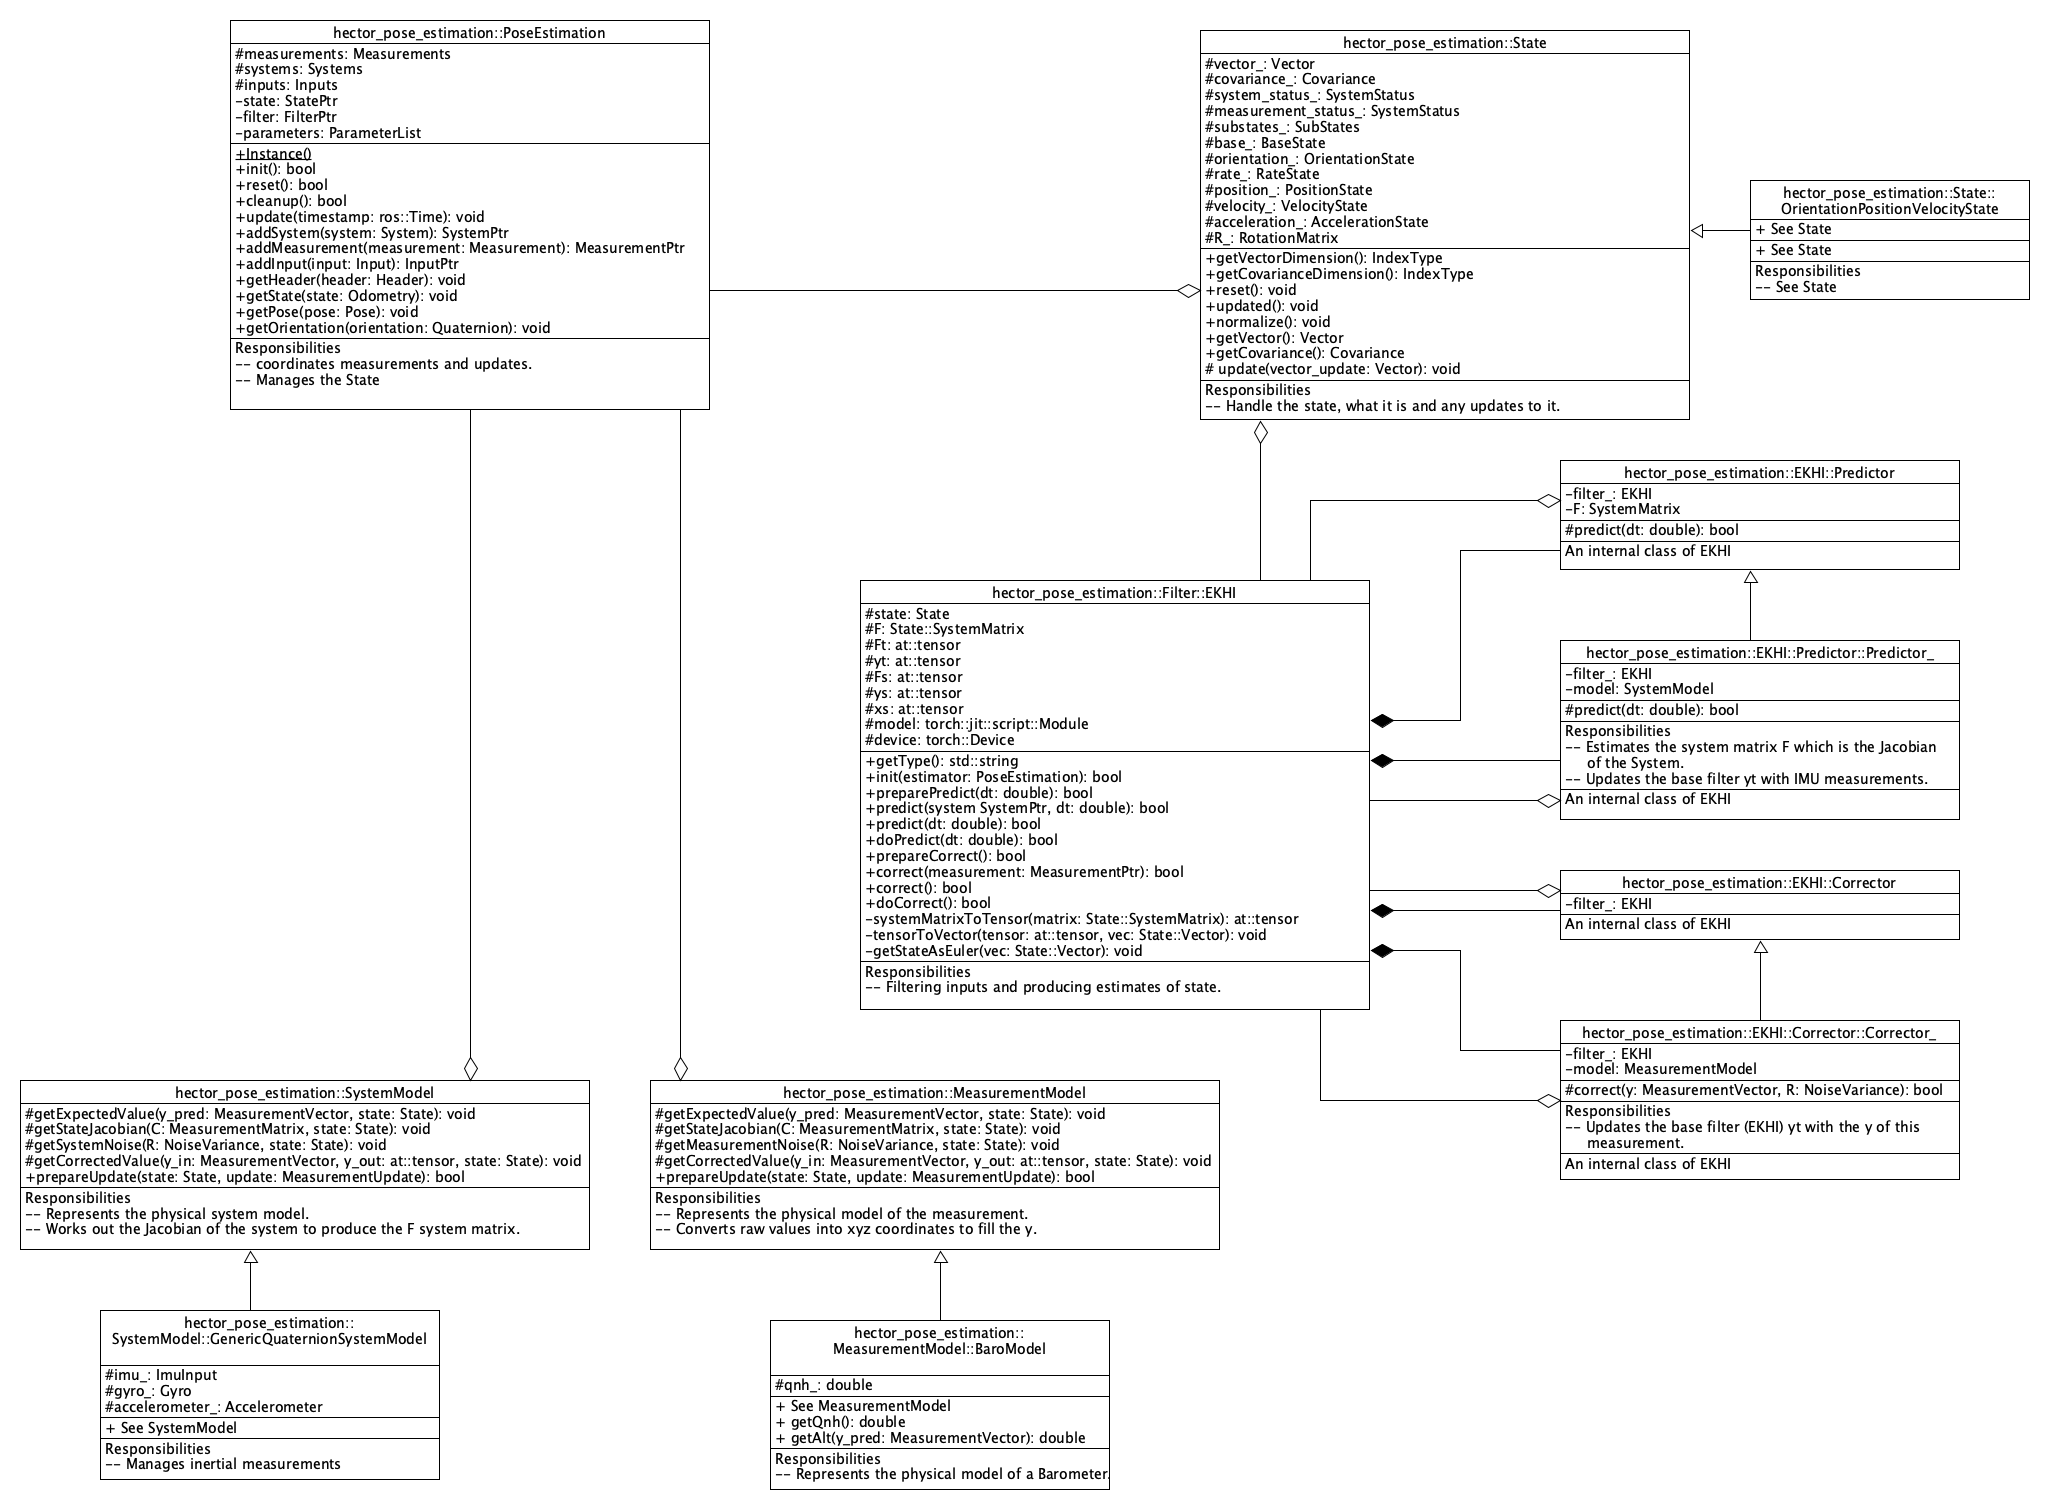
\includegraphics[width=\textwidth]{ekhi_integrationUML.png}  
  \caption{Simplified class diagram of the integration with hector.}
  \label{}
\end{figure}

\begin{figure}[h!]
  \centering
  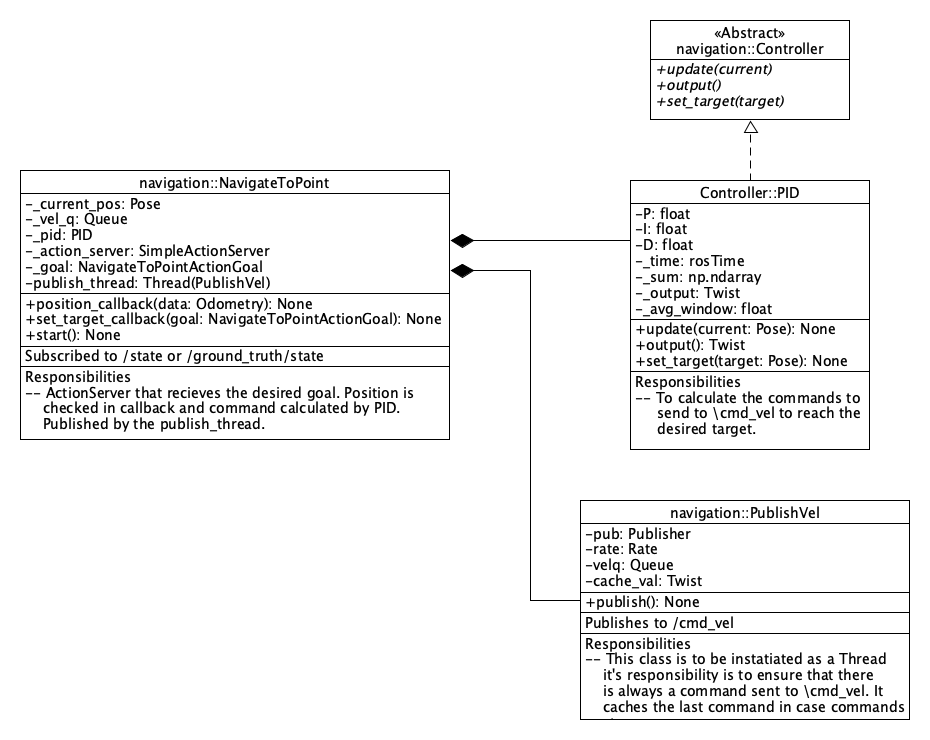
\includegraphics[height=0.4\textheight]{NavigationUML.png}  
  \caption{Class diagram of the ROS control section.}
  \label{}
\end{figure}


\subsection{Testing Strategy}

\subsubsection{Why testing?}
Testing is a critical part of a successful software project and even more so when it will have a long life with revisions and updates. This is true for two reasons, firstly it guarantees certain functionality in the specific situations tested. Secondly is that it guards against releasing regressions.

%% TDD and the advantages
\subsubsection{TDD}
Test Driven Development (TDD) is, at its most simple, the practice of writing tests before writing code. It usually refers to Unit tests though it can apply to all levels of testing.
TDD is the preferred development methodology for a number of reasons. It forces developers to consider the necessary inputs and outputs before writing code. This in turn creates cleaner code with less coupling. At the same time the tests act as an additional form of documentation by defining the acceptable inputs and outputs to functions.

%% challenges to doing TDD in this project
\subsubsection{Challenges in using TDD}

There were unfortunately several challenges in using TDD as the primary methodology. The first is that HI and in general any Deep Learning code is not conducive to direct testing. This is because you cannot tell a priori what the output to a given input is, as this is what you are learning. You can at most verify dimensionality of the outputs.

Also as I was working with and integrating into existing code bases there was often no sensible way to write tests before implementation.

Finally for a lot of the code that dictated behaviours of the quadcopter it is almost impossible to sensibly test it programmatically as the output we are looking for is the movement of the quadcopter.

%% What did I test and how.
\subsubsection{Testing approach}

Given these challenges, I have followed TDD only where it was possible. I have Unit Tested as much of the components as possible while incrementally and continuously testing the integration of the various components while developing. There was a tight cycle of development and testing throughout the project.

While developing the ROS sections I would make changes and then immediately test them functionally, running them in the Gazebo and with debugging output to match the demonstrated function with the output.
The only exceptions to this approach in fact was when there were major refactors that spread across files. In this case I would make a larger number of changes before testing. In all cases of new functionality however I always thouroughly tested each component before moving on to further functionality.

I have thoroughly Unit Tested the components of the proof of concept of HI, the Dataset and Linear Motion model, as well as the extension to accept Inputs and Prediction. The Unit testing proved it's value several times during development when I refactored which introduced some regressions. They allowed me to quickly and easily identify the code responsible and quickly rectify it.

\section{Development}

This section details the process of development that I went through. It is broadly organised by component and within component in chronological order.

\subsection{Hardware}

%% evaluation of alternatives
My original plan was to use a Raspberry Pi (RasPi) for onboard computation for transitioning to operating on the physical drone rather than in Gazebo. This was for a couple of reasons, primary was the low power draw while still offering gigahertz computation. I have a RasPi 2 and I planned to purchase a RasPi 4 for the final implementation due to its increased compute power.

%% selection of Jetson Nano
While experimenting with my RasPi 2 I found some limitations with its implementation of Python as well as concerns about its prospective performance due to reports found online. I researched alternatives, as there are a wide variety of Single Board Computers on the market now. While looking I found that NVIDIA produce the Jetson Nano and specifically the SDK kit, which is very similar to the RasPi but has native support for PyTorch, the deep learning library I am using as well as having 128 GPU cores. This enables me to take advantage of parallelised matrix computation with the associated performance improvements. On top of this it only consumes up to 10W of power, admittedly this is double the 5W draw of the RasPi but 10W is the maximum, not necessarily what it will consume. I planned to explore true power consumption in the second part of the project.

%% installation of PyTorch and ROS.
After the Nano arrived I installed PyTorch and ROS onto it. This allowed me to verify the steps needed for installing both packages and ensure the most streamlined set of instructions.

\textbf{PyTorch Challenges}

There were some issues with the original version of PyTorch installed due to the Nano using an ARM CPU. This means that it has the aarch64 architecture and so compiled executables are trickier to get hold of and often are not quite the same as x86. In this case PyTorch uses some external libraries for some of the matrix operations, these include OpenBLAS and MKL. In the first version I installed these were not present, preventing matrix inverse operations. This is critical to both Graphical Kalman Smoother and by extension the HI implementation.

I tried a number of solutions including installing from source however in the mean time an updated version of PyTorch was released for the Nano which included OpenBLAS solving the problem.

In the end there were a number of factors that prevented the eventual hardware integration.

% I will still try and profile the time and power requirements of running the code for SLAM.

\subsection{ROS and Gazebo}

%% install ROS and Gazebo
The first task to carry out was to install ROS and Gazebo. As mentioned earlier ROS is the framework into which my code will fit. Gazebo is a simulation tool that I will be using to verify everything before deploying anything in reality. Luckily Gazebo is included with ROS (with some exceptions) so installing it separately is not necessary. If you need the most recent version of Gazebo this is not true, you need to follow some additional steps to install it and link it with ROS so they interact correctly.

\pagebreak
I did have some confusion about which version of ROS I needed to be compatible with various things but I made the decision to stick with the most recent version of ROS and the standard version of Gazebo packaged with that. This simplifies the setup for anyone seeking to reproduce this project.

The ROS website\cite{melodic/installation/ubuntu} has an excellent guide on installing ROS for the first time on Ubuntu and I highly recommend it.

%% install hector code
\textbf{Hector stack installation}

After that I installed the hector stack. This was quite a long process of trial and error as there does not seem to be a guide for getting started with this set of packages. I first tried to install them from apt as they are available there. That did not work and I believe the issue is that they were built for an earlier version of ROS but packaged for melodic without any changes. Regardless of the reason that did not work. I was trying to install the hector quadrotor and hector gazebo packages as those were the only packages that I believed that I needed. I tried to clone them into the src folder of my catkin workspace. While trying to build it failed because of dependencies on other hector packages, namely hector slam hector models and hector localization. Then it was missing the geographic mesages. Then it failed because it was missing qt4. I installed both of those with apt. The full process took a while longer than this explanation as you only find out another dependency is missing after building again. A final issue was that the memory usage at certain points spikes. It turned out that this was causing the VM to run out of memory and stop compliation. This caused very confusing error messages as they didnt seem to be for anything in particular. I finally figured out with the help of htop and allocated more memory to the VM which solved the issue. One anachonism of this stack is that it doesn't seem to build in the right order. It will often fail only to complete more after rerunning. At one point it was necessary to continually rerun catkin\_make about 7 or 8 times in a row. The only cause for concern is when it stops at the same percentage built more than once. 

\textbf{Controlling the Drone}

In order to control the drone I decided to use a PID controller as it is standard in robotics and in fact in control in general. There were a couple of issues encountered during this stage, the first was that I decided to use a separate thread to continually broadcast the commands to the \textbackslash cmd\_vel topic which controls the drone. This is to avoid gaps in commands, if the drone does not receive commands it begins to fall due to gravity. I was publishing in this thread at 20Hz. The PID controller is a callback subscriber that runs at the speed of the topic it subscribes to. In this case it is Gazebo and runs at 100Hz. I was using a queue for inter-thread communications but it was blocking when full. This meant that the commands would be dropped, and the published commands would be quite out of date by the time they were published which led to very poor performance. Once diagnosed I reduced the size of the queue and most importantly increased the rate of publishing to \textbackslash cmd\_vel to 100Hz to keep them mostly in sync.

%% youtube link?

\textbf{NAN issue}

There was also a small issue with commands containing nan values. This turned out to be due to the time elapsed between calls to the controller sometimes being approximated to 0. This caused division by 0 issues. This was solved by simply not considering any call with time change of 0.

Once the core PID controller was functioning properly I implemented a ROS Action Server on top of it to navigate the drone to a specified point. This was then used to create a script for specifying particular flight paths. This is in order to demonstrate the drones ability to fly accurately specific paths for comparison.

\subsection{Monocular SLAM with scale recovery}

Unfortunately due to implementation details and incompatibilities that resulted from those, I was unable to use this technique in the final product. I have still included a description of the work carried out for completeness.

%% Go through the process. Look at the diary.
The first step in working with the TUM code was to compile it. I was aware that it was written to target ROS Fuerte with some modifications to support Indigo which is 3 versions behind Melodic.

\textbf{Ardrone\_autonomy challenges}

I first attempted to build the project on the Jetson Nano as I was planning to use it as my development platform as well as the deployment environment if possible. This was not possible. The build failed due to a dependancy, ardrone\_autonomy. This is a wrapper for the Parrot AR drones SDK. It also provides a number of message definitions. I attemped first to build the dependancy on the Nano but there are issues with compiling that code on an ARM platform. This prompted me to drop the dependancy and the speed of compilation prompted me to abandon the Nano for development.

I found that the only code from the ardrone\_autonomy package were the messages. I then extracted the message definitions from the ardrone\_autonomy package into my own package.

\textbf{PTAM challenges}

After solving that issue I ran into much more serious issues with a third party library called libcvd which is an OpenCV alternative that PTAM, the monocular SLAM component. This package is packaged as a thirdparty library inside a tarball with two other libraries. Upon building it would fail on apparently legal C++ code. I tried to use the most recent version of libcvd, pulling it from github, building and installing it on the system separately. This didn't work so I tried placing it into the thirdparty tarball. That also did not work. I found that the directory structure of the new version did not match the original and there was a Makefile I needed to replicate. I then found that there were some files that had been deprecated but the TUM code relied upon so I pulled them over from an old version of the library. This on it's own did not fix the issue but when I found a final Makefile I could add the files I had pulled over into the list of artifacts that would be made available by that stage of the build. 

\textbf{Namespace, tf and GUI challenges}

Then I found some namespace issues as another dependency was not being found in the expected manner. I had to set a definition in order to fix that problem. I also had to remove the GUI section of the code as it had more serious persistent issues. If I have time spare after completing the project I will go back and try and fix that as well. Finally there was a section of code that relied upon 'tf', which is a geometry package of ROS but is now deprecated. I had to rewrite that section to use 'tf2' which is the replacement for 'tf'.

After building it ran without issue. I then explored how to get it to interact with the hector stack. I looked through the hector stack and it is very large. A lot of it is not needed for this project so I considered extracting the core functionality that I want, create a world with a quadcopter that acts correctly. Unfortunately the hector stack has a large number of interdependencies so it is infeasible to extract only certain components.

\textbf{Interation with hector stack}

After deeper examination I found that the architecture of the two projects effectively precludes interconnection. The core of the problem is that they have been designed and built as standalone projects without much concern for modularity. There are good reasons for this, primarily is the need for low latency in pose estimation to ensure effective control. Though this does not preclude a more modular approach, the easiest mechanism to achieve it, ROS nodes and topics, is too heavy weight and would add a lot of latency as well as other potential issues. Unfortunately that means that an adapter is impossible.

\subsection{Hybrid Inference}

%% Create the dataset
\subsubsection{Data}

% understand the linear models, create one
A prerequisite for any task that includes neural network is collecting or creating the data for it to train on. For the proof of concept the dataset is created to firstly verify that the technique works as expected and I can implement it.
I first needed to formulate a simple linear dynamic system that resembled the dynamic system in \cite{Satorras2019CombiningGA} so that I could have some comparison. I decided to use a 2 dimensional dynamic system with only position and velocity. The decision to be made is in the format of the $\bar{x}$s and $\bar{y}$s, which then influences the transition and measurement matrices, $F$ and $H$. To clarify and avoid confusion, $\bar{x}$ and $\bar{y}$ refer to state and measurement respectively and $x$ and $y$ refer to axes of motion. $T$ refer to the $\Delta t$ between time steps.

\begin{align*}
  \bar{x} &= [x, vx, y, vy]\\
  \bar{y} &= [x, y] 
\end{align*}
\begin{align*}
  F = [[1, T, 0, 0],\\
       [0, 1, 0, 0],\\
       [0, 0, 1, T],\\
       [0, 0, 0, 1]]
\end{align*}
\begin{align*}
  H = [[1, 0, 0, 0],\\
       [0, 0, 1, 0]]
\end{align*}

This specification for a linear model is then used with a seed state, number of timesteps, starting point and $T$ to generate a sequence of datapoints. I then created the Dataset class that generated the data and returned it. This is the PyTorch wrapper that allows Dataloaders and simplifies training. I then created a script to return training, validation and test dataloaders.

I later created another model and Dataset for a linear system with inputs. This included a function for generating inputs per time step. I created a simple default that created a periodic, non linear motion.

\textbf{Serialising from C++}

After this I needed to gather data from Gazebo to train the final model, this turned out to be more complicated than expected and I delayed a little until after I had integrated the EKHI into the hector stack. This was so I could return the exact data that the model would see in the real environment.
There were two main challenges to this step. The first was saving the measurements and then loading them into Python. My first thought was to serialise them manually but then I remembered that LibTorch has some serialisation functions that should work with PyTorch, simplifying everything. 

\pagebreak
I originally wanted to use

\begin{verbatim}
  torch::save(tensor)
  torch.load(path)
\end{verbatim}

in C++ and Python respectively but I found that using torch::save in LibTorch didn't work with torch.load in PyTorch 1.3.1 and 1.4.0, it threw an error, I found a work around, which was to use torch.jit.load in PyTorch which gave me a ScriptModule where the named\_parameters were the tensors I had saved.

\textbf{Ground truth}

Then I needed to record the ground truth values for labels to train the model. This required subscribing to the $\backslash$ground\_truth$\backslash$state topic provided by gazebo. The complication was that it was not synchronized with the rate that the pose\_estimation node ran at. This would lead to subtle timing differences that I wanted to avoid. Originally I sped up the ground truth topic and then only kept ground truths of times when the measurements were being recorded.
After some searching I found that the rate of publishing was defined in hector\_quadrotor and the hector\_quadrotor\_gazebo package. There was an xacro file that defined the update rate as 100 Hz. I increased it to 1000 Hz.
Then I processed the recorded data, dropping any unneeded ground truth data and renaming the remaining so that they line up correctly with the measurements.
I later found that I could set float update rates for the world so I set the step size to be 0.01s and the rate to be 0.1. This resulted in an effective real time factor of 1000 while also keeping all updates in sync. This removed the need to post process.

Then I created a Dataset for it. It reads in all the data at once to have it in memory to speed training. This would not work for very large datasets but for this case it should be fine, the largest dataset I worked with was only 20,000 samples and took less than a MB of memory. Again it was necessary to define the creation of Dataloaders for the training, validation and testing sets.

%% Create the Kalman filter
% understand and formulate
\subsubsection{Graphical Model, GNN and Hybrid Inference}

My original understanding of the Hybrid Inference formulation was that the graphical model was a regular Kalman Filter and the GNN was formulated in a similar fashion. As I describe in the Background Theory section that is not the case. The graphical model is a reformulation of the problem and solution. I realised this after reading the paper with reference to the GitHub repository with their implementation \cite{vgsatorrasgithub}. It took a fairly long time to understand their code as it is not really documented and has a somewhat confusing structure.

Implementing the graphical model was then relatively straightforward though trying to keep it self contained and modular complicated things slightly. My implementation of the GNN is quite problem specific. At the moment I can't see much way to make it more generic. Given that I will have to reformulate for the reasons just stated I will explore where the commonalities are and whether a generic version is feasible or desireable. It differs quite a lot from the Satorras' formulation mainly due to my desire to improve the interpretability of the code and give a cleaner flow and structure. Functionally they are equivalent except that my node model is a 3 layer feedforward network whereas the one they implement is 2 layers. I also decided not to implement different modes for graphical only or GNN only as I specified these as separate standalone, or semi standalone in the case of the GNN, classes. As I had implemented the two components separately it made the Hybrid Inference class very simple as it is just a composition of the two.

\pagebreak

At the start of the second term I focused on the HI section of the project. I first sought to verify the results of the HI paper before continuing with solutions to the challenges identified at the end of the first term. Namely that of inputs and that of prediction.

\textbf{Diagnosing poor accuracy}

Firstly I compared the HI model with the graphical formulation of the Kalman Smoother. Initially the results were significantly worse which is not supposed to ever happen. This triggered an in depth review of my implementation to find the source of the error. Every line was stepped through and evaluated, my initial thought was that the GNN part of the implementation was the most likely culprit. I finally discovered that the cause was the number of iterations that the HI implementation carries out before returning the solution. It was 50 compared with the Graphical Kalman Smoother using 200. Once they were equalised the HI performed better than the Graphical Kalman Smoother.

% That resolved I tackled the prediction problem.
\textbf{Inputs and prediction}

After this point I tackled the first of the issues identified in the first term, which was adding inputs. This was fairly simple due to the fact that the Graphical and GNN sections are completely decoupled. The modification was only to the Graphical model section. I also added a new model for data generation that added inputs to the system.

That done I moved on to implementing prediction. This again was fairly straightforward in terms of engineering. It required a wrapper method that augmented a sequence with a number of $0$ entries for the timesteps that prediction is desired for. The only complication is that for the case with inputs it is required to know the inputs for the predicted timesteps beforehand. In reality this is not too unreasonable for short time periods, which is the predominant use case.

% Then implementing it for the drone case.
\textbf{Transition to Extended Kalman version}

In order to train the instance for the simulation there was some minor modifications required to the due to the fact that it is an EKF that we are using in this case rather than a KF with a static transition matrix. The difference is that the transition matrix in this case is a set of differentials that are recomputed at each time step so we need to change the transition matrix $F$ at each time step.

Thankfully due to the way that PyTorch implements it's tensor operations it didn't change too much. It involved passing in a sequence of $F_t$s one per time step rather than having one static $F$ and then reworking a few tensor multiplications to work with the new dimensions.


%%%%%%%%%%%%%%%%%%%%%
%%% Integrate with hector
\subsubsection{Hector Integration}

%%% Torch script 
Due to the architecture of the hector stack it was necessary to directly integrate the HI implementation into the hector\_pose\_estimation\_core module as an implementation of the Filter class. This meant converting the model to be able to run in C++ or calling Python from C++. After analysing the options working in C++, rather than calling Python was best, mainly because it would remove a lot of overhead and thus latency from the evaluation process.

\pagebreak

\textbf{TorchScript Serialisation challenges}

Converting to TorchScript is the mechanism provided by PyTorch for this purpose. There are two methods, tracing and scripting. Tracing is where you provide model inputs (ie. the same dimensions that you would expect) and call trace on the model with those inputs. The tracing involves following or tracing, hence the name, the inputs through the model and constructing an compute graph based on that. This only works for some classes of model and none that contain any dependence on the inputs. For these more complicated cases scripting is the technique to use. That is more in depth and doesn't require inputs. It parses the modules involved and creates the compute graph in that way. I had to use this technique. There are many unsupported features both of Python but also some from PyTorch that I had to remove, and there were some simplifications to control flow that were required to enable compilation. I also had to separate models for use cases with inputs and those without \cite{torchscript}.

%%% C++
\textbf{Errors in forward in TorchScript model}

The next challenge was loading and executing the model in C++. This I expected to be fairly simple given the example code from a tutorial on getting started with TorchScript and C++. Unfortunately that turned out not to be the case. I had issues in executing the forward method of the model. I wasn't able to see any useful debug messages so I spent some time compiling LibTorch in debug mode so that I could get them. Once I had them it was really easy to find the issues. They were all related to unsupported functions in the compiled module and I just had to switch to supported versions. For example
\begin{verbatim}
  new_list = list()
\end{verbatim} 
is not supported for creating an empty list, instead you must use
\begin{verbatim}
  new_list = []
\end{verbatim}

Once fixed I had to manage the inputs to the HI. This meant collating measurements into a single measurement vector and again into a sequence of observations. I first needed to turn raw measurements like pressure or magnetic flux into $xyz$ coordinates for position, orientation or velocity. This was quite challenging for all but the GPS measurements as they were already in the correct format. After figuring that out I needed to assemble a full scale $y$ in the base filter. This is a significant diversion from the EKF implementation that hector uses. They update the state with each individual unconverted and unaccumulated measurment. This was not possible given the structure of HI. I had issues with accumulating in the same way that the transition matrix is accumulated as the Correcter and Predictor though appearing very similar have subtly different interfaces. In the end I directly accessed the base filter from the Correctors and updated the $y$ directly. This is not the approach I favour but it was the only available.

\textbf{Numerical instability}

I created the equivalent HI model in PyTorch and converted it to TorchScript as before. I then had to deal with numerical instability that was causing nan value outputs from the HI model. This turned out to be due to very small values in the $Q$ matrix signifying very little noise. The issues is that the inverse of $Q$ is used in the graphical model so these small values turn into huge values and when multiplied cause unreasonably large output numbers. I increased these numbers by a constant factor to solve this. This means increasing the amount of uncertainty in the transition but this is not unreasonable.

\pagebreak

\textbf{Computational performance and attempt to accelerate}

I found that the performance of the HI model was significantly worse than the EKF which intefered with the ability to compare them. I decided to accelerate the model with a GPU using an AWS instance. This was quite challenging as most things in this section were. I first tried to run the gzserver instance on the server and run the gzclient on my VM. This needed setting environment variables for IPs. This didn't work for unknown reasons.
I then tried to use something called gzweb that sets up a webserver to serve the UI, making it accessible with a browser. This also failed due to dependency versions. It seems that the resources for this is out of date. Finally I tried the original approach but over a VPN. Originally using AWS features to set up the VPN, but this turned out to be excessively complex so I decided to try just using OpenVPN itself. This turned out to be fairly simple and the only modification needed was that the server had to be run locally and I end up using the AWS instance only for the pose\_estimation node. This is to prevent issues with the location of models on the local machine. I needed to convert the code to run on the CUDA device available which was fairly simple however it did expose some issues.

\textbf{Eigen issues hanging}

I found that there was a segfault occuring when my model ran on the CUDA device. After some research I found that it was the Eigen library causing it. It turns out that you cannot pass Eigen matrices by reference without risking subtle bugs that only manifest in some environments. I rewrote the code that I had written to only pass by reference which fixed that issue but exposed another. The pose estimation node would hang seemingly forever when on CUDA but otherwise not. I decided that it was not worth the extra time to debug this issue as I had also figured out how to run Gazebo in slow motion. 

\textbf{Real Time Factor}

Gazebo world files have the option to specify the physics attributes of that world. This includes the size of time updates and how often they update in the real world. The combination of these two allows you to set a new real time factor (RTF). I originally set the step size to 0.001 and real world update rate to be 1 for 1000 times slow down. I later chose to switch to update step size of 0.01 and update rate between 0.1 and 10 depending on whether I was recording data or running pose estimation with EKHI.

\textbf{Format and zeroing issues}

I realised that the format that I had chosen for the ys and xs was different from the representation used by hector. They had orientation followed by position and velocity then rate and acceleration and I had orientation followed by rate then position, velocity and acceleration in xyz triples. This meant that the Fs calculated would not be applicable in the EKHI. I changed this which actually simplified some code at the same time. I found that the majority of the ys were all zeros which was not supposed to be what happened. I had specifically decided that measurements would propagate through time, even if they were a little out of date. I found that the base implementation of getCorrectedValue that I had written zeroed the y tensor. I had not seen any other measurements being used other than the ones that I had overridden this base implementation. I discovered through this that there were a large number of measurements that were called but never had updates.

\textbf{More numerical issues}

I then focused on resolving the appearance of really large numbers in F. I found that after less than quarter of a second several parts of F would contain numbers in the order of $10^5$. I was fairly certain that this was causing EKHI to run into numerical limits and output nans. There were a few dead ends that I had to go down, including ideas about the update to the States covariance matrix but eventually I found that the cause was the getJacobian method in the GenericQuaternionSystemModel. This uses the Accelerometer and Gyro models to compute the F and they add a bias to the value they get from the raw\_imu. This bias was the one that was increasing exponentially in fact, doubling at each time step. I then found that this bias was linked to the State itself which was also increasing exponentially. Finally the root cause was the fact that I was computing the difference between the EKHI prediction and the current state but in the wrong order considering how the update function worked. So every update was pushing the state further away from the estimate. 
 
\textbf{Incorporating IMU data and reducing measurement dimension}

This process did give me a much more full insight into the working of the pose estimation code. I found that the IMU data, rather than being a measurement was treated as an input and directly added to the state. I was then overwriting it and losing all that information. I then added to the predict function to make it add the IMU data to the base filters y which would then be used in the correction stage. I also realised that as there were several axes of motion for which I could not get measurements for the model was only seeing zeros in those positions. This could constrain the model as they are in the place of measurements that though noisy should have some information. I refactored and resized the measurement vector y to be of size 11 rather than 15 but fully filled.

\textbf{Training}

I then focused on examining the impact of training on the performance of this EKHI. To quantify it I used a standard loss function, Mean Squared Error (MSE) loss which calculates the mean of the squared error or the difference between the predicted state and the ground truth. Having gathered data from Gazebo I was able to do this outside of the simulator, on AWS for some acceleration of the EKHI.

Ultimately I was not able to achieve the level of stability of control that I was looking for and so I did not compare side by side the EKHI and the EKF while controlling the quadcopter in Gazebo. I did however learn huge amounts about this new techique and its suitability for this kind of application. I also learned about the challenges of integrating new techniques into existing solutions and the challenges of control and real time computing.

%%%%%%%%%%%%%%%%%
%%%% Results
\chapter{Results}

\section{Results}

The key results are regarding the computational effeciency of the technique and the accuracy.

\subsection{Computational Performance}

This is the most dramatic and obvious result of this project. At the outset I had expected Hybrid Inference (HI) to be a more computationally expensive technique than the standard Extended Kalman Filter (EKF) due to its use of Neural Networks on top of normal matrix operations. I had not expected it to be quite so expensive in terms of time however.

Over many runs in the simulator as well as for training and evaluation, the full scale model with 15 x 15 transition matrices took on anywhere from 0.7 seconds to 4 seconds to run on a laptop CPU. The real surprise was that GPU acceleration did not make that much difference. On a g4dn.xlarge AWS EC2 instance which has an NVIDIA T4 GPU with around 8.1 TFLOPS of performance only improved execution times to 0.35s. 

The reason for this is primarily the graphical underpinnings of this technique. It reformulates a sequential iterative process to one of iterative improvement over a sequence. The number of iterations needed was around 200 for reasonable performance which is a large constant factor to add to an already computationally expensive set of operations. There is somewhat of a trade off here in that you can use less iterations but the accuracy is worse. This does also seem to be highly implementation specific, \cite{Satorras2019CombiningGA} used only 100 iterations in their implementation but for mine that was too low for good performance.
It is unlikely that this form of the technique will be suitable for real time operation without serious reformulation.

\subsection{Accuracy}

The second and more disappointing result was that of prediction accuracy. The performance of the predictor was very variable. As I have mentioned earlier it seems to be fairly tethered to any measurements that it has and will not stray too far away from those. That is fine when they are good but not great where they are very noisy or biased. In addition it seems to be fairly poor at estimating values for those dimensions where it has no measurements. The orientation estimates were consistently poor leading to significant control instability.

I am fairly sure that these issues are tied to the graphical model and its implementation. And it shows that this technique that fuses the advantages of two different approaches to inverse problems is still very sensitive to the formulation of the solution. 

\pagebreak

\subsection{Training}

The final area to remark upon is the effect of training on the performance of the model. This is an area that the model did show positive results. 

As the graph shows there is a clear improvement throughout training finishing out with a 41\% improvement over the untrained performance with training over 2000 samples. 
This is consistent with the results shown in \cite{Satorras2019CombiningGA} in the Lorenz Attractor experiment. It does seem that this technique provides the most benefit to these highly non-linear problems. Their results suggest that with training on up to 10000 samples could see still more improvements. However analysis of the training curve appears to show a settling of the error at a pretty consistent level consistent with approaching the optimal error.

An area that would be interesting to explore would be how robust these results are to poorly formed underlying graphical models. It would be very interesting to quantify the amount of extra training to get to similar levels of predictive accuracy.

\begin{figure}[h!]
  \centering
  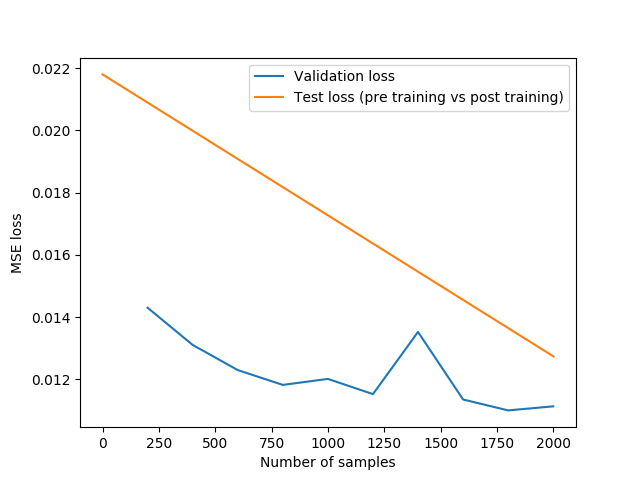
\includegraphics[height=0.4\textheight]{training2000.png}  
  \caption{Results of training Extended Kalman Hybrid Inference}
  \label{}
\end{figure}
\pagebreak

\section{Self Evaluation}

\subsubsection{How did the project go?}

I think that the project went reasonably well, I wouldn't say that it went any better because there were several places where it could have gone better. I did encounter a number of non-trivial difficulties that I had not anticipated and I definitely was too ambitious with my initial project scope. Having said that I think that I managed to implement a solid piece of work that I am proud of. I think that I have also been able to contribute something small to the field by evaluating a new technique in a new application area and that is probably the thing that I am most proud of in terms of what I achieved.

I think that as a learning experience it was hugely valuable, much more so than any of my previous projects to date. The demanding scope of the project as well as the fact that it cut across a number of sub-domains of Computer Science enabled me and really pushed me to learn a lot. I have learned so much about dealing with VMs, Ubuntu as an operating system, ROS and Gazebo programming, PyTorch, LibTorch, TorchScript for developing, training and deploying neural network models.C++, working with CMake and catkin as build tools. Yet more about integration and testing, dealing with remote servers, setting up builds and deployments to be more streamlined, setting up a VPN and some of the vagaries of AWS. I spent a lot of time reading and understanding fairly complex code, mostly from academic sources which gave me an appreciation of the different approaches taken for those particular projects. After this project I feel much more equipped to be a useful member of a development team than I did at any point before.

And although I didn't get to the point of hardware integration, I still learned a lot through the process of preparing for it, both in terms of specifying hardware, exploring potential interfacing issues and some of the challenges of working with low cost compute platform. These generally run ARM chips and so have more complicated requirements in order to work with much of the software which this project is based on. This experience was invaluable and will serve me well into the future.

\subsubsection{Where next?}
% Where next? submitting to DASC.
I have submitted an abstract to the Digital Avionics Systems Conference 2020 (DASC 2020) and I am awaiting notification of whether it is accepted which I will hear on the 25th of April. If it is positive then I will be adapting this report to be an academic paper for publication in that conference. Aside from that I am keen to improve the predictive accuracy to the point where it can sustain stable flight as well as exploring ways to improve computational performance.


%% What did you do right/wrong?
\subsubsection{What did you do right/wrong?}

I think I did quite a few things wrong. As I talked about earlier I was overly ambitious in terms of what I wanted to achieve. This was compounded by the fact that my estimations for how long tasks would take were quite far off. I should have been much more thorough in evaluating the prospective components that I was planning to integrate, though this is more apparent in hindsight. I did spend a fair amount of time evaluating them at the start but I didn't know enough about how they would all fit together until I had worked in and with them for some time to realise the issues that I would have.

As for what I did right, I think that my work output was good and consistent which is quite important to me. Making progress every week makes a big difference to progress overall. I certainly think that I did well in understanding and implementing a cutting edge technique that is not trivial by any means. I also think I adapted fairly well to the changes in the project. It is fairly common in industry that requirements change and circumstances dictate a different approach to the original plan. Adapting to what was possible and scaling back the ambition was the right decision. I also think that the quality of the code that I produced was good and well documented.

\subsubsection{What have you learnt about doing a project?}

I learned a number of important things about doing a project. They fall into three categories.
\textbf{Planning and execution:}

%% Waterfall vs agile
One of the key takeaways for me from this project was about the challenges of trying to apply the Waterfall methodology to software projects. This project was broadly structured as a Waterfall project (though not explicitly) which bled over to the execution. I realised that at the start of a project it is extremely hard to forsee many of the issues that will arise and therefore it is hard to plan for them. This is less applicable for projects that the individual or organisation has carried out a few times before as that prior experience will mean that they will be much more able to anticipate potential issues up front. For example creating a web app for a new customer will have differences but if you have developed several before you will be very familiar with most of the technologies as well as the potential pain points. For this project that was not the case as all of the technology was new to me. 

%% time estimation, ambition and scope
Closely related is the issue of estimating the amount of work required for any specific feature. This was clearly important as the entire project is planned out at the start so any miscalculations can drastically affect the total amount of work required.  I am reminded of a guideline that experienced developers use to evaluate the estimates of less experienced developers of multiplying the number by 2 and incrementing the unit, so for example an estimate of 1 hour becomes 2 days. I understand much better why this is often true. Being that I was working with new technologies it was much harder to estimate these things before getting started and that is one of the main things I learned about estimating timings. The amount of uncertainty in an estimate is inversely proportional to the amount of experience you have with the technology and solution you are implementing.

Having said all that, I have learnt that the most common pain points are in the interface of different technologies and components and often the devil is in the detail. I now know to dive into much more depth at the outset of a project with that in mind to try and find as many pain points up front and think of alternatives and options. That still won't be perfect but it should help reduce issues in the future.

\textbf{External components and academic code:}

%% academic code
A large proportion of the external code that I interacted with is academic code, this provided me with some interesting insights into the differences between academic code and commercial code. Also between different kinds of academic code. For example, the hector stack is structured much more like commercial code, with similar structure and coding standards from what I have seen. In contrast the code related to the HI paper has all the hallmarks of prototype code. This makes sense in context, the code for that paper was written to support a paper and had no particular ongoing application. This removes the need for maintainability or extensibility and even to some extent keeping the code clean. 

%% interfacing issues and details

\textbf{Personal development:}

% consistency
I also learned more about how I deal with working on a large project alone for an extended period of time. It can be hard to maintain motivation at times with a project of this length when working alone.Part of the reason for this is that when working with others, progress is often much faster, others completing different parts of the whole so you can get vertical slices completed quicker. This is helpful for motivation as you see results early and often. When working alone, this is often less true and managing momentum is really important.

% fixing issues
I also realised some of the challenges of maintaining schedules when running into issues during development. While it is often reasonably easy to estimate the time required to complete a feature when the process goes smoothly, when issues arise it is extremely hard to predict how long it will take to solve. Some issues are solved in a matter of minutes, whereas others can take days to work through. Often the time taken is related to how much assistance there is available either online or in person. For the majority of application development there is a large amount of knowledge available online to refer to when encountering difficulties. Unfortunately for me ROS and Gazebo have more limited communities using them. And when implementing new techniques, there is no reference other than the paper, and maybe source code if made available via GitHub. This forced me to work through most issues alone. While this slowed development significantly, I would say that it did improve my troubleshooting skills significantly.

%%%%%%%%%%%%%%%%%
%%%% BIBLIOGRAPHY

\newpage
\bibliographystyle{acm}
\bibliography{../resources/final_project}

\label{endpage}

\begin{appendices}

%% Project Diary
  \chapter{Project Diary}

  Monday October 7: Learned about ROS topics and publishers. Created two simple example programs. One to make a simple robot travel in a circle, one to stop. Appears that publishing once to the /cmd\_vel topic does not have any effect. Appears that it needs to be sent multiple times.
  
  Wednesday October 9: I set up the git repo both on my main device and the VM in which I will be working mostly. I added the Project Plan to the Reports folder and generally did some repo management.
  
  Saturday October 12: I have started my report on Kalman Filters. I have read the important parts of the original paper introducing the technique as well as some other explanations. I have written the introduction.
  
  Sunday October 13: I started reading the follow up paper to the original Kalman paper which expands on the technique. I also spent more time understanding the mathematics of the original paper.
  
  Monday October 14: I learned more about publishers and subscribers. I created my catkin workspace. I am having some issues in setting up my development environment how I want it. I want to have ros and gazebo running concurrently and interacting but I am not sure how to get that working. That will be the next thing to work on.
  
  Thursday October 17: I worked on getting the hector\_quadcopter package working. This will be my base for experimentation and work. This took a lot of time and pain. Getting the correct packages in the right place was not simple. This is mainly because the most recent version of ROS and Gazebo are not supported as standard. You have to clone 4 of the tu-darmstadt repos and repeatedly call catkin\_build. One major hiccup I encountered was that at one stage the memory needs expands dramatically and can cause a non-obvious failure. I will detail more on the best installation procedure in separate notes.
  
  Saturday October 19: I finished my report on Kalman Filters. Right now it seems a little too high level so I may return and add in the mathematical content.
  
  Monday October 21: I learnt more about how to connect the Raspberry Pi to the Matrice 100. I found that it is somewhat easier than I expected in some ways and a bit harder in others. There is a cable to connect from the UART on the drone to USB on the RasPi. However I will need some kind of voltage regulator for the power supply. In addition, the interface between ROS on the RasPi and the Matrice and DJI OSDK is not clear yet.
  
  Wednesday October 23: I learned more about Services and how to write Service clients and servers in rospy. I also learned some about writing ROS packages in C++. I think that I will probably end up writing packages in C++ due to performance requirements for my project. I am planning to write demonstrators in rospy and use that to determine whether that will be sufficient. If not I will implement the final deliverables in C++.
  
  Thursday October 24: I reevaluated the project plan, assessed progress so far and revised my milestones for both terms. This has led to a more organised structure to the plan, with more focused proof of concept programs and a more logical structure to second term deliverables. I have now organised them around the implementation details ie. hardware, software or data.
  
  Monday October 28: I started learning about Graph Neural Networks. I found a couple of review papers that should contain a good overview as well as references to specific techniques.
  
  Tuesday October 29: I continued learning about Graph Neural Networks. I have decided to review an online guide that introduces the basic concepts before continuing with the academic papers.
  
  Friday November 1: I started to prepare a Raspberry Pi (Raspi) to run PyTorch and ROS. I updated the version of python to 3.7 which was more effort than I expected due to the way Raspian deals with python. I also researched alternatives to the Raspi in case it is not powerful enough (quite likely). I have decided the best alternative is the Nvidia Jetson due to price (100 pounds) and the fact that it has cuda support which will speed up code execution by a significant factor. It is also compatible with PyTorch out of the box which will simplify my life considerably.
  
  Monday November 4: I finished learning about ROS Actions so I know have all the pieces I need to implement my project from the perspective of ROS. I read the GRIN paper in full so I now have a good idea of what I will be implementing from that point of view. Finally I also learned about PyTorch Geometric which is what I will use to implement the GNN part of the algorithm. I still have much more to learn on that part but I have a good start at this stage.
  
  Wednesday November 6: After meeting with Sara I looked at which version of ROS the TUM code is targeting or working with. It is Indigo so it is likely to need a reasonable amount of work to port to Melodic. I have also decided to push back the report on Graph Neural Networks as it is too broad at this point. I will refocus the report and complete it after one exploring more of the professional issues as well as a report on GRIN, the technique I am looking to implement.
  
  Thursday November 7: I rewrote my Project Plan today to take account of the changed scope and deliverables anticipated. I also finished a first draft of the report on GRIN.
  
  Sunday November 10: I set up the Jetson Nano device. I installed ROS, Gazebo and PyTorch. This means that it is now ready for deploying code once I have integrated it with the Matrice. I also set up my project, cloning and building the libraries that I am using. This was again painful but now I know the pain points I have written a clear and simple guide to getting it up and running.
  
  Thursday November 14: I have forked the TUM repository that I need to port to the current version of ROS and then extend. I attempted to build it on the Jetson Nano. It failed due to a dependency on a package called ardrone\_autonomy. I attempted to install that to satisfy the dependency but it failed. It seems that it can’t be built for ARM architecture which is a problem. It is mainly a wrapper for the Parrot AR SDK. I tried on the VM I have on my laptop as it is amd64 architecture so that would avoid the issues with ARM. It failed for other reasons that seem to require rewriting the library. I abandoned this. I then tried to find all the references to ardrone\_autonomy in the TUM code to remove them. There were not too many. So I decided to replace them where possible.
  
  Friday November 15: I found that most of the references to ardrone\_autonomy are just using messages defined in the ardrone\_autonomy package. I found the definitions and extracted them into a new standalone package called navdata\_msgs. After some work on the CMakeLists.txt file and package.xml it builds successfully. I then replaced all occurences of ardrone\_autonomy with navdata\_msgs. On building I get other errors related to a third party library that the TUM code relies upon. This is called libcvd and it seems to fail on C++ compliant code which is confusing. I tried removing the library from the tarball that it is packaged in and install it from source elsewhere but this still fails. I now know that because I was not cleaning before remaking it was using a cached version so no changes were propagated to the new build.
  
  Saturday November 16: I have tried again to incorporate the new libcvd into the thirdparty tarball. The new version makes fine on its own so I hope that it will be fine if I get the configuration correct. I found that the original had a different folder structure as well as a Makefile that the new one (from GitHub) did not. I replicated the old structure and tried to rebuild and it gets much further than before but now gets stuck linking a header file from the new libcvd. I had to pull over two old files from libcvd-1.0 thread.h and runnable.h as they are used in the TUM code for some reason, it doesn’t affect any other code so it is safe to do this. Also add \#include to cvd/utility.h to fix another bug in the new libcvd version. Currently it doesn’t think that transform is part of the CVD namespace though it seems to be defined to be so in cvd/vision.h. Need to figure that out. This whole process is somewhat exemplary of the difficulties of using old academic projects. There are often serious compatibility issues because they are not maintained. This is the main challenge at this point. Once everything has been built successfully this will hopefully be less of an issue as I can control what is modified and build upon what I have learned about the project structure and CMake. Pretty useful experience though in terms of debugging old make configurations. I had no idea about how CMake worked or how to use it but now I have a pretty good idea.
  
  Sunday 17 November: I finished my report on the applications of GPS Denied Navigation. I fixed the error of transform not being defined in the CVD namespace. It turns out that you need to have CVD\_HAVE\_TOON defined for that function to be defined in the header file. After defining it before import it then works. There is another issue though of Thread not referring to anything as I needed to move the thread.cpp file at the same time as thread.h. Currently having issues in linking the moved files. Getting pretty close to having it work I think though.
  
  Monday November 18: I added the thread header and source files to the CMakeLists.txt. But it didn’t work. I tried to make install TooN. That didn’t work as there was no target for install. Then I tried switching to libcvd 1-x branch. Didn’t work. I removed the GUI Node as I don’t need it and it was causing problems that are not easily reconcilable, potential solutions caused new issues. I found that no thread files or functions were becoming part of the .so file (shared object). From that I found a Makefile I hadn’t looked in before, it was inside libcvd, that added all the .o object files. I added cvd\_src/thread.o to the list and it worked. Added roslib to the CMakeLists.txt and package.xml as it has been separated from roscpp and is needed by one of the functions. Refactored EstimationNode.cpp and .h to remove references to tf and use tf2 instead. This was the final issue as tf has been deprecated. I also had to add tf2 to the dependancies list in CMakeLists.txt. After all that I now have the TUM code building successfully. It took much more time than I wanted but that is unfortunately part of the process. If I had reimplemented it all myself, I would have saved time in debugging build errors but spent much more time in development overall. I think that despite the work it should be worth it. Next is to test the functionality and interface it with the hector drone.
  
  Thursday November 22: I ran the TUM code and it runs with no errors at this point. I started to review the hector stack to see how I can interface the TUM code as the SLAM and controlling node. The hector stack is very large and has lot’s of interdependencies. I am exploring the feasibility of porting the core elements to a package that has less coupling. This is for two reasons. One is to enable the project to be set up more simply and enable easier extension. Second is to reduce overhead so the Jetson has an easier job compiling and running the code. I have not come to a decision yet as it will be non trivial to accomplish due to the interconnectedness.
  
  Saturday November 24: I familiarised myself more with the hector codebase. I have decided that it is not a good idea to try and extract the minimal core elements. The code base is simply too large and interconnected to do in a reasonable amount of time. I will instead modify just one of the packages to interface and work with the TUM code. I have also been thinking about the correct way to incorporate these projects into my github setup. Currently I have forked the repositories that I need to modify and I was planning to add them as submodules but I need to consult Dave to see if that is acceptable. There are alternative solutions that keep all of the project private if that is necessary so I will do that if I need to after consulting Dave.
  
  Sunday November 24: I got the date of the last post wrong. On Sunday I spent more time learning about Graph Neural Networks. I have also found that there is a Distinguished Lecture on the topic of Graph Neural Networks on Monday so I will be going to that and I shall see if it improves my understanding. I will be starting to implement the GRIN this week as well as writing a report on Graph Neural Networks so the timing is very good! I am also starting my interim report in order for it to be mostly complete by the end of the week ready for Sara to read and give feedback on a draft.
  
  Tuesday November 26: I created the dataset for the GRIN or Hybrid Inference implementation. I needed to define a linear model that will generate the data for a simulated system. The maths was not too involved, the only complication is in the discretisation of the equations. After defining the linear model, I added a function that generates a number of samples, returning the ground truth (state) and the measured position. The next step is to define the Kalman filter and then the Hybrid Inference setup. Then training and testing. I am behind schedule but I still expect to complete on time due to the slack I built in to the schedule.
  
  Saturday November 30: I worked out the formulation of the Hybrid Inference technique. This took me a lot more time than expected as I had previously understood that it consisted of a Kalman filter and an additional GNN. That is not actually how it works. They reformulate the Kalman filter as a graph message passing routine that passes messages from past states, future states and observations in order to iteratively improve the estimates of the states. The GNN is then an equivalent graph that has hidden states of x replace x (states). These are randomly initialised. The hidden states of y are the y’s (observations) passed through either a convolution or an MLP to generate the hidden states of y. The picture is of the white board where I worked this all out. I referred to the paper for most of the graphical formulation. For the GNN part I referred to the source code that the authors wrote in addition to the paper. Neither are particularly understandable so there was a lot of referring back and forth and figuring out what was meant.
  
  Sunday December 1: I wrote my own implementation of Hybrid Inference. I referred a lot to the workings I had done on the whiteboard the day before. The GNN implementation was still the most opaque part of the whole technique. There are quite a few tricks and I was trying to write it in a more modular fashion to facilitate using it standalone for comparison purposes. I am not sure that I achieved it but it is at least close and structurally it is modular. I know that it will need some modifications before it will work correctly on its own but they should be minor. The GNN step is something of a mirror of the graphical formulation with the matrix multiplications that compute the messages between nodes replaced by 3 layer neural networks. Then a neural network computes the new hidden states of x and finally in the hybrid formulation there is a decoding step that creates a correction signal epsilon that helps to modify the estimates of x better than the graphical model alone. Testing is the next step to verify that it works as expected followed by training and evaluation.

  Wednesday December 4: I wrote the training script for Hybrid Inference. I am currently using the Mean Squared Error for the final estimate. This is different to the implementation in the paper and may be changed in the future. Training does not take too long for small datasets of around 1000 samples, taking only 10 minutes per epoch on a CPU. For full training I will be using a GPU instance for acceleration. At the same time I evaluated the speed of individual evaluations over a test set of 500 samples. It took just under a minute which equates to around 0.1 seconds per evaluation on a CPU. This is promising though not perfect and further evaluation needs to be done on the deployment target, the Jetson Nano.

  Thursday December 5: I finished writing the Interim Report and submitted it along with the code to this point. I wrote a brief README that explains project setup and directory structure. I also created a presentation for the Interim Review and submitted it via Moodle. I covered the core motivations of the project and Hybrid Inference in detail. I am a little light on details of work completed but this is mostly due to time constraints and the fact that my project is implementing a fairly new technique so I feel it needs more explanation.

  Saturday January 18: I worked out the maths for adding input to the hybrid inference model. I wasn’t able to work fully through the derivations so I will need to verify everything experimentally. That will be the focus of this week.

  Monday 20 -Thursday 23 January: I have been trouble shooting issues with training on CUDA (GPU). This is to figure out the best parameters for training the network. I have also spent some time thinking about the best approach to adding the input. I have decided after fully verifying the basic network to add some simple input, a simulation of forces that should push the position in a circle. After that I will work on implementing the system for use in drones. This will not be simple and requires some more research as to how DJI represents the drones state.

  Friday January 24: I fixed all of the CUDA issues. The final issue was due to a tensor creation op in one of the component models that was being done on the CPU instead of the CUDA device. I set up training on an AWS instance but it is currently taking 10 hours + to train and the results are not satisfactory. I will add batch training support to speed training and then evaluate the reason for the poor performance.

  Monday 27 – Tuesday 28 January: I have implemented batch support. I had to create a specialised version of the GRUCell for this as the two options in PyTorch, the GRU and the GRUCell don’t allow me to do what I need to in this case. It is currently a very simple implementation and is likely to be a bottleneck in training. I will evaluate this and rethink if necessary. The weighted loss function that I need to test is still to convert to work with batches, that will be the next bit of work.

  Friday January 29: I trained HI with the weighted loss as well as bog standard MSE. The weighted loss performed slightly better and didn’t show any particular performance loss in training so I will stick with it. I also found that a smaller training set size seemed to perform better. I am not quite sure why at this point so I will continue to try and evaluate and diagnose that.

  Monday February 3: I implemented the new HI model that accepts inputs into the linear dynamic system. This now needs to be tested to evaluate it compared with the non input model.

  Tuesday February 4 to Friday February 7: I modified the evaluation methods to enable comparison between HI and the Graphical version of the Kalman Filter. This is to evaluate whether HI is better than the Kalman Filter.

  Saturday February 8: I modified the training to operate over more samples and less epochs. I evaluated different models of HI with and without input against Kalman filter implementations. They were consistently worse. Somewhat strangely there were identical results for HI trained with different training hyper parameters.

  Monday February 11 to Wednesday February 13: I wrote the Professional Issues section of my Final Report. I focused on the potential applications of autonomous drones. It does require review and improvement.

  Saturday February 15: I reviewed some literature on Graph Neural Networks to better understand where my implementation may have gone wrong. I read through a good review of all GNN approaches and related them to the paper on HI.

  Monday February 17 and Tuesday February 18: I stepped through my implementation line by line and related it to the HI paper, my understanding of GNNs and the implementation of the authors of the HI paper, in an effort to diagnose the cause of the poor performance. I found that the inputs to the edge accumulator networks were not what they should have been. In my next post I will detail the differences. I have fixed these issues as well as averaging issues in the evaluation function. Next is to test whether the changes have solved the performance issues.

  Wednesday February 19: The differences found on Monday and Tuesday were not the issue though they did need fixing. I discovered today that the error was originating in the graphical section of the HI. The GNN part could not overcome this. This was caused by the number of iterations being far too low at 50 compared to the just graphical kalman filter using 200. After equalising these HI is better even with no training.

  Friday February 21: I verified that the same fix for the regular HI worked with the extension to inputs. I still need to compare with a regular non graphical kalman filter.

  Monday and Tuesday February 24 and 25: I wrote self-evaluation, and graph neural network background theory sections. I also reworked the work completed section to add work completed this term. The professional issues section was completed on the weekend and worked into the report. The draft is completed and sent to Sara for feedback.

  Tuesday and Wednesday March 3 and 4: I implemented a comparison with a regular Kalman Filter, including converters between data types and the evaluation method.

  Friday March 6: I added prediction to HI as well as adding Smoother and Predictor classes to improve the class structure and aid extensibility.

  Monday March 9: I wrote a Controller abstract base class for Controllers to inherit from, enforcing certain methods. I wrote an implementation of a PID controller that should provide instructions to navigate to a point. I wrote a publisher thread that continually publishes to /cmd\_vel. This is necessary to avoid the drone from falling, it needs constant instruction. I put them together to test them. There were some issues in control, the drone did not get to or stay at the desired point.

  Tuesday March 10: I fixed the issue with the drone not being controlled properly. I also overcame some issues in the PID controller. Due to the ground truth publishing at around 100Hz but not exactly, sometimes the time between measurements is 0. This causes division by 0 issues resulting in nan instructions which is a problem. Solved by ignoring updates with 0 time difference. The issue causing the drone to not be controlled properly was twofold. First was that the publisher thread was publishing at 20Hz and the PID thread was running at ground truth speed or 100Hz. As I am using a Queue for thread safe communication it filled up very quickly and caused lag issues. Increasing the publish rate to 100Hz has solved the issue for now and I am working on a sensible way to avoid the problem altogether. I refactored the PID section to use ROS Actions and implemented a proof of concept that can fly particular shapes or flight paths between specified points.

  Wednesday March 11: I tuned the PID controller and tested it using both ground truth and hectors own pose estimation for positioning. There is a noticeable difference, as I expected in position holding stability and accuracy. I started looking for where hector implements the Kalman Filter in their own pose estimation part.

  Thursday March 12: I spent a long time looking for the Kalman Filter. One of the challenges of working with code written with ROS and in particular this set of packages, is that the relationships between modules and pieces of code is extremely tricky to discern sometimes. Because nodes can communicate via topics in this case theres no direct link between files, so you have to use some ros tools to try and find which nodes are using which topics and then find which piece of code creates that node. It is a little bit of detective work. In the end I found that the EKF is created in the hector\_pose\_estimation package which is then imported and added to in the hector\_quadrotor package. Not a very obvious link so it took quite a while to find it.
  Friday March 13: I spent time understanding the implementation of the EKF in hector\_pose\_estimation\_core. It is a somewhat complicated implementation subclassing a base class of Filter with two internal classes, Corrector and Predictor. The most confusing part is the extensive use of templating to define types, the fact that there seem to be implementations of Corrector and Predictor known as Corrector\_ and Predictor\_ and finally the fact that the EKF class seems to be passed in to it’s own internal classes. Then there are also methods for augmenting the Filter and adding measurements.

  Saturday March 14: I started to draw up the HI implementation, based on the EKF implementation that I explored on Friday. As part of that I converted the model to TorchScript so that I can load it into C++. I had to use the torch.jit.script method for this rather than torch.jit.trace because the HI model has various aspects of control flow in its forward method that are incompatible with tracing. I found that I had to remove almost all type hinting as the compiler could not interpret it correctly. I also removed the possibility of changing the number of iterations in the forward method and fixed it at 200. I removed as much as possible dimension checks as well. I managed to load the model into C++ but had errors in the forward pass.

  Monday March 16: I spent more time trouble shooting the forward pass of the model. This is extremely challenging. There are essentially no resources for this issue. The C++ interface of PyTorch, also known as LibTorch is very sparsely documented but more importantly not very used so there aren’t many people who have had similar problems, or ideas for troubleshooting. I did find someone with somewhat similar symptoms who had been advised to rebuild while setting debug, this is because there is no stack trace, or easy way to print the error as it is C++. I tried to rebuild with debug enabled but it made no difference. I decided to use CLion to help with debugging and it did help me identify what is going on, though not the reason for it. The problem seems to be that the model cannot find a method called forward, this is odd because when I evaluate it step by step, it hits the line that should return the method but then skips over it and returns an error instead.

  Tuesday – Friday March 17 – 20: I spent these days finalising the vast majority of the report, tidying and improving sections. Making sure that it flows well and that it is understandable with little context. Having been through the process, I have found that my explanations sometimes make assumptions based on that experience, that others will not have. This rewrite has I think corrected most of that and now I would say that barring a few final touches and corrections the report is essentially complete. I sent a copy to Sara for her feedback.

  Saturday March 21: I implemented the Extended Kalman version of HI. The main difference is in the fact that the transition matrix F is now a sequence of matrices, one per time step. It is passed into the forward method rather than specified for the class. This required some rewriting of matrix multiplications in the graphical model. I also verified that the reformulation is functionally the same as the original with the same matrix at each time step.

  Monday – Thursday March 23 -26: I spent the start of this week trying to understand the implementation of pose estimation in hector. This was much more work than I had anticipated mostly due to the design decisions of the hector team. They have extensively used templating and inheritance, I do understand to some extent why they structured it the way they did, to increase extensibility from an architectural point of view. The main issue is in understanding the code sufficiently to actually extend it and add a component. The data flow is extremely complex and not obvious, the entire span of calls to update the state crossing at least 9 files and jumping up and down inheritance hierarchies. The real problem here is that there is no documentation at all and the code is not particularly readable, a fair amount of which is probably due to use of language features that I am not familiar with. After much time spent I mostly understand the flow necessary to integrate HI into the package.

  Saturday and Sunday March 28 and 29: I worked on setting up the work flow for the Extended Kalman Hybrid Inference (EKHI) integration with hector. The work flow is quite different to the EKF that is already there and I realised that I spent too much time trying to understand what they were doing instead of just understanding the structure enough to implement EKHI within that structure. There are several challenges in integration. The first and most challenging is the structure of the data. The measurements y that I have been modelling to this point were the entire set of measurements all at once. In this case there are multiple different measurements at different times. Assembling a consolidated y is challenging as there is no real information as to what exactly the measurement is modelling, whether acceleration or velocity etc. A second challenge is that the pose estimation predicts position much more often than correcting it. This is tricky mostly because the state transition matrix F is calculated every predict but measurements come only with every correct. That is a problem mainly because the graphical nature of HI really needs one transition between measurements not multiple. There were two options to overcome this, one is to just use 0 vectors for the ys of predict steps. The other was to accumulate the effect of the transitions by matrix multiplying the transition matrices at each predict and using the consolidated F for the correction. I opted for the second approach as I feel the resulting model will be more accurate rather than using so many 0 vectors. There is still a potential for inaccuracy in the predict step as the time step involved will not be constant. I will evaluate this on completion and try the alternative if performance is poor.

  Monday to Friday March 30 – April 3: I first worked on assembling full size ys to put into the EKHI model. Firstly I had to figure out what each of the measurements applied to in the state space. I formulated my state space as [orientation, rate, position, velocity, acceleration] in groups of xyz for each. This is different than the representation used by hector. For some reason I don’t fully understand, they use a 15 vector, the same size as I do, but they selectively use only some of the entries. For this specific application they only use orientation, position and velocity but they occupy the first 9 slots of the vector, and the rest is random numbers. I knew that the baro measurement was an indirect position z measurement. I had to figure out how to convert it to actually represent that. That took quite a while. Then I had to do the same for the magnetometer reading. This was much more challenging as the built in methods of true heading and magnetic heading often did not tally at all to the orientation z element (yaw), which is what it should be similar to. I realised that those methods were minusing the existing yaw from the measurement. This was giving a difference but not an absolute measurement. I added a additional method to get the absolute converted reading. Finally gps, which was much simpler as it already gave absolute measurements. For some reason the ekf does not seem to process any imu data, at this stage I am not sure whether that is because they are using some other filtering technique, no filter (which would be very odd), or because they are not used in the current setup. After figuring out these issues, I needed to find a way to update the global y that will actually be inserted into the model. This was much more challenging than I had expected. The structure of the predictor and corrector are extremely similar and give the impression that they both informally implement a kind of interface. This is not the case. The base filter cannot access the corrector the same way that it can access the predictor. I tried a few fixes to equalise the implementations so that I could keep my code consistent. Unfortunately each of these broke significant parts of the rest of the hector package so I abandoned them. Finally I found that I could directly update the global y in the corrector as I had access the other way round. This is not my preferred implementation but I am working within rather tight constraints. Finally I started working on the final pieces of the EKHI flow, calculating the difference between the models output and the current state. I encountered some unexpected behaviour, with debugging print statements not printing as expected. I made the decision to rebuild from scratch which then failed with new errors that I had not experienced before related to the version of LibTorch that I had built in order to get debugging. After rebuilding LibTorch and that doing nothing, I abandoned debugging and switched back to the prebuilt binaries which allowed the project to rebuild successfully. It also seems to have solved the printing issue.

  Monday April 6: I finished implementing the EKHI integration bar final testing. I fixed the calculation of updates, converting from tensors to Eigen Matrices and updating the state. I also formulated the noise matrices for the model. There was a small hiccup in that the actual matrices have 0s on the diagonal, which means that they are singular matrices and therefore not invertible. This is a problem because matrix inverses are essential to the graphical formulation of the Kalman Filter. I added a small epsilon (1e-9) to make the model work but I do need to see if this affects performance. I also ran into some problems in the predict step. This is because although I can export a function from the PyTorch model which will then be present in the TorchScript model that I load in C++. The issue is that the compiler has no idea which methods have been exported in that particular model as it is loaded at runtime so it causes compilation errors. I looked for ways around this but there was essentially no information on the subject. I decided to bring the functionality of the predict function into the hector EKHI integration, as it is quite straightforward. I just add 0s for the final y and call the regular forward function, so no big deal.

  Tuesday April 7: I fully function tested the integration of EKHI. I fixed a few bugs, some in the integration, some in the formulation in PyTorch. One example is the fact that the model is frozen when scripted into TorchScript. If the model is in training then all the modules that have different configurations will run with those. This was a problem for the batch norm layers. I also found that because the model is set up for batch training the inputs need to be in batches. This required unsqueezing the inputs (adding an outer dimension). I also found that the EKHI implementation is incomplete and needs batcherizing for the Fs. The main takeaways from today was the need to improve the performance both in speed of execution as well as accuracy. I am running into numerical issues with nan s being returned. I suspect the state noise matrix Q as many of the entries are very small. See the earlier post on the reasons for some of those. I will troubleshoot and hopefully fix these tomorrow.

  Wednesday April 8: I tried several methods of improving performance. I started by profiling the code. This involved some modification to launch files so that I could run the pose estimation node separately. I also had to install perf which is what CLion uses for profiling C code. I had some issues, the most major of which was that after 10 – 40 seconds (it seemed to vary mostly based on the rate of sampling) my laptop would crash. I am not sure exactly why this happened but I suspect it is to do with interactions between perf, Ubuntu, VMWare and MacOS. I did manage to get some useful data eventually, learning that a huge amount of time was being wasted creating huge numbers of threads. I rectified this by running the code with the environment variable OMP\_NUM\_THREADS=n. This improved performance by a small amount.

  Thursday April 9: I decided to set a baseline for the performance to compare the performance in C++ to. I ran an equivalent EKHI in plain PyTorch as well as a version compiled to TorchScript. They both had very similar performance to the LibTorch implementation. I also found that the main determinant of performance is the number of iterations that the algorithm updates. This presents a direct trade off between accuracy and performance. At 200 it is accurate but slow and at 50 it is fast but inaccurate. It is possible that I can improve the tradeoff with some parameter tuning so that it arrives at the optimal estimate in less iterations. I will explore this if there is time available.

  Thursday April 9: Second part. I also explored the numerical stability issues with nans being returned. I first tried removing nans in the conversion from tensor to Eigen. This added resilience as I then got useable values for the rest of the system regardless of the results from EKHI. Then I looked at why EKHI was returning nans. I suspected the small values in Q and I was correct. The smallest value was 1e-9 and when inverted this is quite large, as there are several multiplications this quickly becomes too large to store and the tensor library turns it into nans. I increased the size of each element by 1e4 as this was the first size that the implementation returned non nan output. This corresponds to adding some uncertainty to the transition which is actually quite realistic. This is why I consider it to be acceptable.

  Friday April 10: I decided to try to accelerate the implementation with a GPU. This involves running on an AWS server and forwarding the output to the VM that I have used for most of my development. I tried X forwarding as it seemed like the most straightforward approach. That didn’t work, there was an issue with OpenGL. This was not specific to Gazebo as it was also a problem while running the test program glxgears in the same way. I decided to abandon this approach as it seemed to have something to do with the 3d drivers on the server, which didn’t seem like it would be quick to solve. I then tried to run gzserver on the server and port forward to my local machine where I would run gzclient to show the UI. This did not work either with the UI not ever really showing up.

  Saturday April 11: I decided to explore alternatives to running on AWS to deal with the performance issues. This involves reducing the real time factor (RTF) of the Gazebo simulation. This allows the quadcopter to perform in the sim as if there was more time available for processing, or greater computational resources to speed it up. I found that I needed to change the world file but it was not where I thought it was. I spent some time looking for it and found it in /usr/share/gazebo-9 though this will change depending on how it was installed. I found the empty world file which is the one I am using and added a RTF override. That didn’t work so I changed the real\_time\_update\_rate to be 10 which equates to a RTF of 0.01.

  Monday April 13: I worked more on deploying to AWS. I tried again to use port forwarding with no success. I then tried to use gzweb which runs the server as a webserver, allowing you to see the Gazebo GUI in a web browser. This also didn’t work, there were lots of dependancy issues and the most recent guide was based around gazebo7 and an old version of both nodejs and npm. I finally tried to use a VPN to connect my VM and the AWS instance. Firstly using AWSs built in Site-to-Site VPN, this involved setting up gateways for the VM and Virtual Private Cloud that the instance is within and then connecting them. I wasn’t able to access the VPN and the guidance was a little tricky so I decided to try setting up a VPN from scratch using OpenVPN. The reason I hadn’t tried that before was that I was not sure whether the network settings used by AWS would cause problems. After finding the AWS facilities a little convoluted, I decided that it was worth a try. It turned out to be pretty easy, the only issue is that it needs setting up again from scratch every time I spin up a new instance as the setup is obviously dependant on ips etc. Thankfully it is really easy once you know the steps. After setting that up I was able to run sections on the server and render locally. I was not able to run it all on the server due to issues with model locations. Luckily there is only one node that needs the GPU of the instance so that is pretty easy. I ran it on a non GPU instance to verify that it works. Finally I converted the EKHI hector integrated code to work with CUDA (GPU) support. I will test this tomorrow.

  Tuesday April 14: I edited the majority of my Final Report. I added to testing and improved the wording of many sections. I also added references to several sections. All that remains is to finish off the Development and UML sections and fill in the Results section and then a final review.

  Wednesday April 15: I worked on running the pose\_estimation node on a GPU accelerated AWS instance. I found that the AMI that I had created to reduce setup time had lost all cuda drivers for some reason. So I started from scratch again with a blank Deep Learning Base AMI. This did give me the opportunity to streamline and improve my setup and installation instructions which are now pretty bulletproof given a blank Ubuntu 18.04 VM. I found a subtle bug involving the Eigen library. After porting to cuda, it would seg fault, I ran it with valgrind and it showed an illegal read of size 16 which shouldn’t have happened. I found out that you should never pass Eigen Matrix’s by value, only by reference and that it is often fine but on certain configurations it will show issues. I refactored and tested again but the EKHI would then just hang for no observable reason. I decided that it was not worth the time to investigate much further particularly as the debugging available to me is very limited. Quite a frustrating day.

  Thursday April 16: I worked on saving data from Gazebo to use in testing. The first idea was to serialise manually and write to file but this would have been a lot of work so I looked at serialisation within libtorch and pytorch. I did some searching and it looked like serialisation had been recently introduced into libtorch so you could save in that and then load into pytorch without issue. That turned out not to be quite true. I tested saving in libtorch using torch::save() which seemed to work fine but it would error out when using torch.load() in pytorch. This was the issue I found when I had searched so I knew that I should be able to used torch.jit.load instead. I tried that and it gives you a ScriptModule with the named\_parameters of that being the tensors you saved. That just adds a little annoyance to interacting with them but nothing serious. Once that was done, I added saving to the ekhi model, I had to add a counter so that it would save to separate files. I separated ys and Fs. Then I had to save the ground truths. This was pretty easy as I could do so in Python. I wrote a ROS node that subscribed to the ground truth topic and saved it in a similar way to in libtorch but with no need to use torch.jit.load() when loading back. I had to convert the ground truth messages which are ROS Odometry messages into the same format as the ys. This only had one real challenge which was converting quaternions into euler angles. In the end I used scipy to initialise a rotation matrix from the quaternion and then used one of their methods to get the euler angles. I convert everything to pytorch tensors, concatenate them and save them. I needed to take account of the time to make sure that the ground truths and measurements were synchronised. This was fairly easy as time is accessed by ros time in C++ in microseconds and each Odometry message also contained the time in nanoseconds. I converted them both to milliseconds.

  Friday April 17: I changed the formats of the ys and the outputs from the EKHI to be the same as the states representation, that is xyz triples for [orientation, position, velocity, rate, acceleration] in that order, where they had previously been [orientation, rate, position, velocity, acceleration] this removed a lot of shuffling and meant that the Fs would work correctly in the EKHI. I also ran the first data gathering runs, I found that it was quite easy to just run the regular setup that would use ground truth for navigation. That took a little modification of some launch files. Then I could in another terminal run pose estimation which contained the EKHI but with actual estimation removed for speed in order to record the ys and the Fs. This worked fairly well.

  Saturday April 18: I found that a large number of the ys were completely zeroed out. This was particularly weird because I had considered rezeroing at every timestep but decided against it, preferring measurements to persist to avoid this issue. I did some searching and I found that there were some measurements that I was not using that were being called but very infrequently. Because I had not implemented the method that I created to get absolute values from the measurements, the default method from the base class was running and in there I had zeroed out the y. I removed this and that resolved that issue.

  Sunday April 19: I created Dataset and Dataloaders for the data collected from Gazebo. I did need to manage the times and synchronise the data from the EKHI and the ground truth. Later that day I found that I could change the real time update of Gazebo to use a step size of 0.01 but at a rate of 0.1 seconds per step in real time. This meant that the ground truth was from exactly the same time as the EKHI and removed the need for synchonisation. I wrote evaluation scripts for the training. I also filled in more of the Final Report, added some references where they were needed and did some more polishing.

  Monday April 20: I focused on resolving some issues that were causing certain values in the Fs to become really large. I thought that these large numbers were causing the EKHI to output nans. I knew that this didn’t happen with the EKF and so I thought that it might have something to do with the States P or prior values as that is not something that the EKHI updates. I traced that value and it had no correspondence with the changes to F so that was not it. I found that it was coming about in the GenericQuaternionSystemModel in the getJacobian method, which creates one of the component Fs that gets combined into the final F. I traced through the execution much closer than I had before and I found that the IMU was updating the State directly and that it also formed part of creating F at each predict section. I then found that the gyro and accelerometer readings of the IMU were becoming really large after a short amount of time. I found that this was because the bias in their respective models was increasing very rapidly. There was no clear mechanism for this which was very confusing and made me think that there might have been some updates in the State that were responsible that I had missed. I actually found that the State itself was becoming really large really quickly and that the bias was proportional to the State. I eventually figured out that after the EKHI predicted or corrected, it computed the difference between that estimate and the current state. The order was the wrong way around for the way that the State update function worked as it added the difference. So every update was driving the state away from the estimate instead of correcting it to equal the estimate. I added gravity as a measurement as it seemed to be showing up while collecting data where I had not seen it before. This was a little challenging to work out how to convert it to absolute values for orientation but I found that atan2(y, z) would give me the pitch and -asin(x) gave me the roll. I ended up discarding this measurement because it was very very noisy. I also found that the measurements that the model observed differ depending on whether the model uses ground truth with pose estimation running in another process or whether it uses pose estimation directly. This was true especially for height vs baro.

  Tuesday April 21: I found that the EKHI was not able to predict very well with the measurements that I had. I realised that the accelerometer and gyroscope readings were being discarded because they were directly added to the state before the predict step and the predict step doesn’t use them to predict so those values are overwritten with the models estimation only. So I decided to add them to the measurement vector y and include them in the correction step. I expected this to make a big impact on stability but it did not. One of the challenges of the EKHI model in comparison to the EKF model that it replaces in this instance is that it expects all the measurements to arrive at the same time, that is each vector of measurements should be full and relevant. This is not the case here and for most drones barring some preprocessing. The GPS updates are at 4Hz, the baro is approx 10Hz and the IMU is approx 100Hz. In addition, I had formulated the ys to be the same size as the state, but I was not getting any measurements for orientation. These were then always 0 which restricted the model to predicting values around 0. I decided to resize the ys to only contain measurements which I was reading, this reduced the size from 15 to 11. Unfortunately this didn’t seem to improve model performance in predicting orientation. I found that the model would not stray far from the measurements and so was fairly constrained in how accurate it could depending on the accuracy and coverage of the measurements. This is not the expected behaviour but the original paper only covered fairly simple dynamic systems and only one with changing F matrices. I suspect that the primary issue is with the F matrices as these are the key component of the Graphical Models function. If they are not accurately estimated by the quadcopter then the updates will not improve the estimates. The final thing that I will evaluate is the impact of training both on total error rates in isolation as well as on the stability of the drone in simulation.

  Wednesday and Thursday April 22-23: I worked on tidying up the integration and training the model on an AWS instance. I found that the training was quite effective at reducing the error, it reduced mse by around 40\%. I finalised the report adding the sections on Results and finishing the Development section. I did a final review and tagged a release on GitHub and finally submitted my report and code.
  
\end{appendices}
  
\end{document}

\end{article}